%%%%%%%%%%%%%%%%%%%%%%%%%%%%%%%%%%%%%%%%%%%%%%%%%%%%%%%%%%%%%%%%%%%%%%%%
%DIF LATEXDIFF DIFFERENCE FILE
%DIF DEL /tmp/claude-0/-home-user/177710a6-83c7-584b-8f2f-a9a7012a7684/scratchpad/v8_sent.tex   Wed Nov 11 14:44:19 2026
%DIF ADD main.tex                                                                               Wed Nov 11 14:53:39 2026
% ICDE 2027 research paper (Round 2: submission due 11 November 2026).
% Format rules from the call for papers (https://icde2027.github.io/):
%   * IEEE conference template, PDF only.
%   * At most 12 pages, excluding references and the AI-generated content
%     acknowledgement. No appendix is allowed.
%   * Single-blind review: authors and affiliations are shown.
%   * Every author needs an ORCID at submission time.
%%%%%%%%%%%%%%%%%%%%%%%%%%%%%%%%%%%%%%%%%%%%%%%%%%%%%%%%%%%%%%%%%%%%%%%%
\documentclass[conference]{IEEEtran}
\IEEEoverridecommandlockouts

\usepackage{cite}
\usepackage{amsmath,amssymb}
\usepackage{booktabs}
\usepackage{multirow}
\usepackage{array}
\usepackage{graphicx}
\usepackage{tikz}
\usetikzlibrary{arrows.meta,positioning,fit,calc,shapes.geometric}
\usepackage{xcolor}
\usepackage{enumitem}
\usepackage{xspace}
\usepackage{algorithm}
\usepackage{algpseudocode}
\usepackage[hidelinks]{hyperref}
\usepackage{orcidlink}

\definecolor{sblue}{HTML}{2B6CB0}
\definecolor{sgreen}{HTML}{2F855A}
\definecolor{sorange}{HTML}{C05621}
\definecolor{sgray}{HTML}{4A5568}
\definecolor{spurple}{HTML}{6B46C1}
\newcommand{\system}{\textsc{Synthagent}\xspace}
\newcommand{\best}[1]{\textbf{\boldmath #1}}
\newcommand{\sd}[1]{\,{\tiny$\pm$#1}}
\newcommand{\resq}[1]{\textbf{RQ#1}}

% Figures are produced by generate_paper_assets.py from the ablation run.
% If a figure has not been generated yet, a framed placeholder keeps the
% manuscript compilable instead of failing the build.
\newcommand{\assetfigure}[2]{%
  \IfFileExists{#2}{\includegraphics[width=#1]{#2}}{%
    \fbox{\parbox[c][3cm][c]{\dimexpr#1-2\fboxsep-2\fboxrule\relax}{\centering\small\ttfamily missing asset: \detokenize{#2}\\ run generate\_paper\_assets.py}}}}
%DIF PREAMBLE EXTENSION ADDED BY LATEXDIFF
%DIF UNDERLINE PREAMBLE %DIF PREAMBLE
\RequirePackage[normalem]{ulem} %DIF PREAMBLE
\RequirePackage{color}\definecolor{RED}{rgb}{1,0,0}\definecolor{BLUE}{rgb}{0,0,1} %DIF PREAMBLE
\providecommand{\DIFaddtex}[1]{{\protect\color{blue}\uwave{#1}}} %DIF PREAMBLE
\providecommand{\DIFdeltex}[1]{{\protect\color{red}\sout{#1}}}                      %DIF PREAMBLE
%DIF SAFE PREAMBLE %DIF PREAMBLE
\providecommand{\DIFaddbegin}{} %DIF PREAMBLE
\providecommand{\DIFaddend}{} %DIF PREAMBLE
\providecommand{\DIFdelbegin}{} %DIF PREAMBLE
\providecommand{\DIFdelend}{} %DIF PREAMBLE
\providecommand{\DIFmodbegin}{} %DIF PREAMBLE
\providecommand{\DIFmodend}{} %DIF PREAMBLE
%DIF FLOATSAFE PREAMBLE %DIF PREAMBLE
\providecommand{\DIFaddFL}[1]{\DIFadd{#1}} %DIF PREAMBLE
\providecommand{\DIFdelFL}[1]{\DIFdel{#1}} %DIF PREAMBLE
\providecommand{\DIFaddbeginFL}{} %DIF PREAMBLE
\providecommand{\DIFaddendFL}{} %DIF PREAMBLE
\providecommand{\DIFdelbeginFL}{} %DIF PREAMBLE
\providecommand{\DIFdelendFL}{} %DIF PREAMBLE
%DIF HYPERREF PREAMBLE %DIF PREAMBLE
\providecommand{\DIFadd}[1]{\texorpdfstring{\DIFaddtex{#1}}{#1}} %DIF PREAMBLE
\providecommand{\DIFdel}[1]{\texorpdfstring{\DIFdeltex{#1}}{}} %DIF PREAMBLE
\newcommand{\DIFscaledelfig}{0.5}
%DIF HIGHLIGHTGRAPHICS PREAMBLE %DIF PREAMBLE
\RequirePackage{settobox} %DIF PREAMBLE
\RequirePackage{letltxmacro} %DIF PREAMBLE
\newsavebox{\DIFdelgraphicsbox} %DIF PREAMBLE
\newlength{\DIFdelgraphicswidth} %DIF PREAMBLE
\newlength{\DIFdelgraphicsheight} %DIF PREAMBLE
% store original definition of \includegraphics %DIF PREAMBLE
\LetLtxMacro{\DIFOincludegraphics}{\includegraphics} %DIF PREAMBLE
\newcommand{\DIFaddincludegraphics}[2][]{{\color{blue}\fbox{\DIFOincludegraphics[#1]{#2}}}} %DIF PREAMBLE
\newcommand{\DIFdelincludegraphics}[2][]{% %DIF PREAMBLE
\sbox{\DIFdelgraphicsbox}{\DIFOincludegraphics[#1]{#2}}% %DIF PREAMBLE
\settoboxwidth{\DIFdelgraphicswidth}{\DIFdelgraphicsbox} %DIF PREAMBLE
\settoboxtotalheight{\DIFdelgraphicsheight}{\DIFdelgraphicsbox} %DIF PREAMBLE
\scalebox{\DIFscaledelfig}{% %DIF PREAMBLE
\parbox[b]{\DIFdelgraphicswidth}{\usebox{\DIFdelgraphicsbox}\\[-\baselineskip] \rule{\DIFdelgraphicswidth}{0em}}\llap{\resizebox{\DIFdelgraphicswidth}{\DIFdelgraphicsheight}{% %DIF PREAMBLE
\setlength{\unitlength}{\DIFdelgraphicswidth}% %DIF PREAMBLE
\begin{picture}(1,1)% %DIF PREAMBLE
\thicklines\linethickness{2pt} %DIF PREAMBLE
{\color[rgb]{1,0,0}\put(0,0){\framebox(1,1){}}}% %DIF PREAMBLE
{\color[rgb]{1,0,0}\put(0,0){\line( 1,1){1}}}% %DIF PREAMBLE
{\color[rgb]{1,0,0}\put(0,1){\line(1,-1){1}}}% %DIF PREAMBLE
\end{picture}% %DIF PREAMBLE
}\hspace*{3pt}}} %DIF PREAMBLE
} %DIF PREAMBLE
\LetLtxMacro{\DIFOaddbegin}{\DIFaddbegin} %DIF PREAMBLE
\LetLtxMacro{\DIFOaddend}{\DIFaddend} %DIF PREAMBLE
\LetLtxMacro{\DIFOdelbegin}{\DIFdelbegin} %DIF PREAMBLE
\LetLtxMacro{\DIFOdelend}{\DIFdelend} %DIF PREAMBLE
\DeclareRobustCommand{\DIFaddbegin}{\DIFOaddbegin \let\includegraphics\DIFaddincludegraphics} %DIF PREAMBLE
\DeclareRobustCommand{\DIFaddend}{\DIFOaddend \let\includegraphics\DIFOincludegraphics} %DIF PREAMBLE
\DeclareRobustCommand{\DIFdelbegin}{\DIFOdelbegin \let\includegraphics\DIFdelincludegraphics} %DIF PREAMBLE
\DeclareRobustCommand{\DIFdelend}{\DIFOaddend \let\includegraphics\DIFOincludegraphics} %DIF PREAMBLE
\LetLtxMacro{\DIFOaddbeginFL}{\DIFaddbeginFL} %DIF PREAMBLE
\LetLtxMacro{\DIFOaddendFL}{\DIFaddendFL} %DIF PREAMBLE
\LetLtxMacro{\DIFOdelbeginFL}{\DIFdelbeginFL} %DIF PREAMBLE
\LetLtxMacro{\DIFOdelendFL}{\DIFdelendFL} %DIF PREAMBLE
\DeclareRobustCommand{\DIFaddbeginFL}{\DIFOaddbeginFL \let\includegraphics\DIFaddincludegraphics} %DIF PREAMBLE
\DeclareRobustCommand{\DIFaddendFL}{\DIFOaddendFL \let\includegraphics\DIFOincludegraphics} %DIF PREAMBLE
\DeclareRobustCommand{\DIFdelbeginFL}{\DIFOdelbeginFL \let\includegraphics\DIFdelincludegraphics} %DIF PREAMBLE
\DeclareRobustCommand{\DIFdelendFL}{\DIFOaddendFL \let\includegraphics\DIFOincludegraphics} %DIF PREAMBLE
%DIF COLORLISTINGS PREAMBLE %DIF PREAMBLE
\RequirePackage{listings} %DIF PREAMBLE
\RequirePackage{color} %DIF PREAMBLE
\lstdefinelanguage{DIFcode}{ %DIF PREAMBLE
%DIF DIFCODE_UNDERLINE %DIF PREAMBLE
  moredelim=[il][\color{red}\sout]{\%DIF\ <\ }, %DIF PREAMBLE
  moredelim=[il][\color{blue}\uwave]{\%DIF\ >\ } %DIF PREAMBLE
} %DIF PREAMBLE
\lstdefinestyle{DIFverbatimstyle}{ %DIF PREAMBLE
	language=DIFcode, %DIF PREAMBLE
	basicstyle=\ttfamily, %DIF PREAMBLE
	columns=fullflexible, %DIF PREAMBLE
	keepspaces=true %DIF PREAMBLE
} %DIF PREAMBLE
\lstnewenvironment{DIFverbatim}{\lstset{style=DIFverbatimstyle}}{} %DIF PREAMBLE
\lstnewenvironment{DIFverbatim*}{\lstset{style=DIFverbatimstyle,showspaces=true}}{} %DIF PREAMBLE
%DIF END PREAMBLE EXTENSION ADDED BY LATEXDIFF

\begin{document}

\title{\system: Reliable LLM-Based Synthetic Data\\Generation for Small Healthcare Datasets}

% ORCIDs are entered in the submission system.
\author{%
\IEEEauthorblockN{Sancho Amaral Sim\~oes\textsuperscript{1,*}\,\orcidlink{0000-0001-6013-4754},
Jo\~ao P. Vilela\textsuperscript{1,2}\,\orcidlink{0000-0001-5805-1351},
Pedro Henriques Abreu\textsuperscript{1}\,\orcidlink{0000-0002-9278-8194}}
\DIFdelbegin %DIFDELCMD < \IEEEauthorblockA{\textsuperscript{1}\textit{University of Coimbra, CISUC/LASI - Centre for Informatics and Systems of the University of Coimbra,}\\
%DIFDELCMD < \textit{Department of Informatics Engineering}, Coimbra, Portugal\\
%DIFDELCMD < \textsuperscript{2}\textit{CRACS/INESCTEC-DCS - FCUP, University of Porto}, Porto, Portugal\\
%DIFDELCMD < \textsuperscript{*}Corresponding author\\
%DIFDELCMD < {\small\texttt{sanchosimoes@student.dei.uc.pt}, \texttt{jvilela@fc.up.pt}, \texttt{pha@dei.uc.pt}}}
%DIFDELCMD < %%%
\DIFdelend \DIFaddbegin \IEEEauthorblockA{\textsuperscript{1}\textit{University of Coimbra, CISUC/LASI - Centre for Informatics and Systems of the University of Coimbra,}\\
\textit{Department of Informatics Engineering}, Coimbra, Portugal\\
\textsuperscript{2}\textit{CRACS/INESCTEC-DCS - FCUP, University of Porto}, Porto, Portugal\\
\textsuperscript{*}Corresponding author\\
{\small\texttt{sanchosimoes@dei.uc.pt}, \texttt{jvilela@fc.up.pt}, \texttt{pha@dei.uc.pt}}}
\DIFaddend }

\maketitle

\begin{abstract}
The performance of classifiers trained on small data, common in healthcare, can be improved by adding synthetic records to the training data\DIFdelbegin \DIFdel{. The }\DIFdelend \DIFaddbegin \DIFadd{, provided these do not expose the real patients. However, existing }\DIFaddend synthetic data generation approaches \DIFdelbegin \DIFdel{in the literature, however, }\DIFdelend typically do not address the difficulty of small data: they learn only from the few records available. Large language models (LLMs) bring domain knowledge from pre-training, but their output often \DIFdelbegin \DIFdel{lacks }\DIFdelend \DIFaddbegin \DIFadd{has too few }\DIFaddend records or contains records that do not follow the structure of the real data, with missing, extra or misnamed columns and values of the wrong type or outside the expected ranges, which \DIFdelbegin \DIFdel{silently corrupt the training data . In this context, we }\DIFdelend \DIFaddbegin \DIFadd{must be detected and corrected before the data can be used. We therefore }\DIFaddend developed \system, an LLM-based approach whose control layer checks and repairs every response against the structure of the real data, and can also enforce value ranges, so that \DIFdelbegin \DIFdel{the requested dataset is delivered intact}\DIFdelend \DIFaddbegin \DIFadd{every requested record is delivered with the columns and types of the real data}\DIFaddend . \system was tested on ten healthcare datasets with seven LLMs from two providers and compared with thirteen generators. It was the only LLM-based generator \DIFdelbegin \DIFdel{whose datasets were always intact}\DIFdelend \DIFaddbegin \DIFadd{that delivered every requested record in this form in every completed run}\DIFaddend , achieved the highest fidelity among the LLM-based generators and the largest median F1-score gain of all, and kept a privacy attack near chance.
\end{abstract}

\begin{IEEEkeywords}
small data, synthetic data generation, large language models, healthcare
\end{IEEEkeywords}

%======================================================================
\section{Introduction}
\label{sec:intro}
%======================================================================
Many prediction tasks in healthcare, such as diagnosing a disease or anticipating an adverse outcome, have too little data. A rare disease may have only a few dozen diagnosed cases, a single-facility study is limited to the patients it can recruit, and labelling records often requires expert review. Sharing data between facilities could add records, but privacy regulations often restrict it~\cite{rieke2020digitalhealth}, so each facility \DIFdelbegin \DIFdel{often }\DIFdelend \DIFaddbegin \DIFadd{usually }\DIFaddend has to learn from its own data. We call such datasets \emph{small data}: datasets whose number of records is too low to train a reliable prediction model, a limit that depends on the number of features, the number of classes and the frequency of the outcome~\cite{riley2019binary}. A common remedy for small data, and for a lack of data in general, is synthetic data generation (SDG), which adds to the training set artificial records that follow the distribution of the real ones~\cite{qian2023synthcity}. This paper focuses on SDG for prediction tasks on small healthcare datasets.

SDG is, however, hardest when data are small. Oversampling techniques, such as the Synthetic Minority Over-sampling Technique (SMOTE)~\cite{chawla2002smote}, \DIFdelbegin \DIFdel{and }\DIFdelend deep generative models, such as the conditional tabular generative adversarial network (CTGAN) and the tabular variational autoencoder (TVAE)~\cite{xu2019ctgan}, \DIFdelbegin \DIFdel{learn the distribution from the same }\DIFdelend \DIFaddbegin \DIFadd{and language models fine-tuned on the target data~\mbox{%DIFAUXCMD
\cite{borisov2023great,solatorio2023realtabformer} }\hskip0pt%DIFAUXCMD
learn only from the }\DIFaddend few records they are meant to complement\DIFdelbegin \DIFdel{, recombining }\DIFdelend \DIFaddbegin \DIFadd{. They can therefore only recombine }\DIFaddend patterns that already exist in those records, for example by interpolating between two existing patients~\DIFdelbegin \DIFdel{\mbox{%DIFAUXCMD
\cite[Sec.~2.8]{cover2006elements}}\hskip0pt%DIFAUXCMD
}\DIFdelend \DIFaddbegin \DIFadd{\mbox{%DIFAUXCMD
\cite{chawla2002smote}}\hskip0pt%DIFAUXCMD
, and most were designed and evaluated on datasets with tens of thousands of records~\mbox{%DIFAUXCMD
\cite{xu2019ctgan,kotelnikov2023tabddpm,zhang2024tabsyn}}\hskip0pt%DIFAUXCMD
}\DIFaddend . Large language models (LLMs) \DIFdelbegin \DIFdel{offer another route. They are pre-trained }\DIFdelend \DIFaddbegin \DIFadd{can add what the records lack. Pre-trained }\DIFaddend on large text corpora, \DIFdelbegin \DIFdel{which gives them domain knowledge about healthcare variables, such as plausible ranges }\DIFdelend \DIFaddbegin \DIFadd{they know plausible ranges of healthcare variables }\DIFaddend and typical relations between them, and they can generate new records from a few real examples placed in the prompt, without any training on the target dataset~\cite{borisov2023great,seedat2024cllm}. \DIFaddbegin \DIFadd{This makes them a promising source of synthetic records when data are small.
}

\DIFaddend Their output, however, \DIFdelbegin \DIFdel{is }\DIFdelend \DIFaddbegin \DIFadd{cannot be used directly as data. An LLM returns }\DIFaddend text that has to be parsed into records, and \DIFdelbegin \DIFdel{nothing guarantees that it forms a dataset: }\DIFdelend a response may contain fewer records than requested, \DIFdelbegin \DIFdel{malformed records, }\DIFdelend missing or invented columns, or values of the wrong type \DIFaddbegin \DIFadd{or outside plausible ranges }\DIFaddend (Figure~\ref{fig:teaser}). \DIFdelbegin \DIFdel{For data management, an LLM is thus an unreliable data source: like any automatic data producer, its output should satisfy integrity constraints before it is loaded into }\DIFdelend \DIFaddbegin \DIFadd{Such records cannot be added to }\DIFaddend a training set \DIFdelbegin \DIFdel{~\mbox{%DIFAUXCMD
\cite{ge2021kamino,rorseth2026recovering,schelter2018deequ,breck2019datavalidation}}\hskip0pt%DIFAUXCMD
. Two integrity constraints apply: the dataset must have the configured number of records, and every record must have the columns of the real data with values of the right type. First, }\DIFdelend \DIFaddbegin \DIFadd{as they are. A missing column or a value such as }\texttt{\DIFadd{age="sixty"}} \DIFadd{stops the training job or becomes a missing value, and a shortfall defeats the purpose of augmentation: }\DIFaddend the number of synthetic records is \DIFdelbegin \DIFdel{a design decision, usually a proportion of the real training set chosen , for example, }\DIFdelend \DIFaddbegin \DIFadd{usually chosen }\DIFaddend to balance the classes~\cite{chawla2002smote}\DIFdelbegin \DIFdel{; }\DIFdelend \DIFaddbegin \DIFadd{, so }\DIFaddend a generator that returns 64\% of them leaves the minority class under-represented\DIFdelbegin \DIFdel{, which is the problem augmentation was meant to solve. Second, synthetic records are typically loadedinto a training pipeline without inspection, where a missing column or a value such as }\texttt{\DIFdel{age="sixty"}} %DIFAUXCMD
\DIFdel{either stops the job or is silently turned into a missing value. Moreover, datasets of different sizes cannot be compared fairly across generators or runs, nor exchanged between facilities in an agreed format . A generator that violates these constraints thus corrupts the training data without the user noticing. In addition, each request to a commercial LLM has a monetary cost, proportional to the tokens (word fragments) processed}\DIFdelend \DIFaddbegin \DIFadd{. Like the output of any automatic data source, these records must satisfy integrity constraints before they are loaded~\mbox{%DIFAUXCMD
\cite{ge2021kamino,rorseth2026recovering,schelter2018deequ,breck2019datavalidation}}\hskip0pt%DIFAUXCMD
. Approaches that prompt an LLM, such as CLLM~\mbox{%DIFAUXCMD
\cite{seedat2024cllm} }\hskip0pt%DIFAUXCMD
and EPIC~\mbox{%DIFAUXCMD
\cite{kim2024epic}}\hskip0pt%DIFAUXCMD
, focus on prompt design and on selecting the generated records, and constrained decoding, offered by LLM providers, fixes the format of each response but not the number of records; none ensures that the requested dataset is delivered. Finally, because the records describe patients, the synthetic data must not reveal the real records used to generate them}\DIFaddend , which is \DIFdelbegin \DIFdel{rarely reported}\DIFdelend \DIFaddbegin \DIFadd{the reason for generating data instead of sharing the real data}\DIFaddend .

The problem \DIFdelbegin \DIFdel{is therefore how to obtain from an LLMa synthetic }\DIFdelend \DIFaddbegin \DIFadd{addressed in this paper is therefore to generate, with an LLM, synthetic records that improve classifiers trained on small healthcare data, delivered as a }\DIFaddend dataset with the \DIFdelbegin \DIFdel{configured }\DIFdelend \DIFaddbegin \DIFadd{requested }\DIFaddend number of records \DIFdelbegin \DIFdel{, }\DIFdelend \DIFaddbegin \DIFadd{and }\DIFaddend the columns and types of the real data\DIFdelbegin \DIFdel{and a known cost that can improve classifiers trained on small data}\DIFdelend \DIFaddbegin \DIFadd{, and without exposing the real patients}\DIFaddend . Formally, given the training records $D$ of a small dataset, their columns and types $S$ and the \DIFdelbegin \DIFdel{configured }\DIFdelend \DIFaddbegin \DIFadd{requested }\DIFaddend number of synthetic records $N$, a configuration $\theta$ of the generator produces a synthetic dataset $G_\theta$. The goal is to find a configuration whose dataset belongs to the set $\mathcal{F}(S,N)$ of datasets with exactly $N$ records that conform to $S$ and that maximizes the gain in classifier performance $\Delta U$, while keeping the distance from the real distribution $L_{\mathrm{fid}}$, the privacy risk $L_{\mathrm{priv}}$ and the cost $\kappa$ low:
\begin{equation}
\theta^{\star}\in\operatorname*{arg\,min}_{\theta:\,G_{\theta}\in\mathcal{F}(S,N)}
\bigl(-\Delta U,\;L_{\mathrm{fid}},\;L_{\mathrm{priv}},\;\kappa\bigr)(\theta).
\label{eq:multiobjective}
\end{equation}
$\mathcal{F}(S,N)$ encodes two integrity constraints, the requested number of records and the columns and types of the real data~\cite{wang1996beyond,batini2009methodologies}, and the objectives are the utility, fidelity and privacy on which synthetic data are evaluated~\cite{qian2023synthcity,lautrup2025syntheval}, together with cost: $\Delta U$ is the change in classifier performance when $G_\theta$ is added to $D$, $L_{\mathrm{fid}}$ the divergence between the real and synthetic distributions, $L_{\mathrm{priv}}$ the success of a membership-inference attack, and $\kappa$ the number of tokens processed; Section~\ref{sec:setup} defines how each is measured. The objectives are kept separate rather than combined with weights, because the right trade-off depends on how the data are used; \system satisfies the \DIFdelbegin \DIFdel{constraint }\DIFdelend \DIFaddbegin \DIFadd{constraints }\DIFaddend by construction and is compared with other generators on the objectives.

\DIFdelbegin \DIFdel{Deep generators~\mbox{%DIFAUXCMD
\cite{xu2019ctgan,kotelnikov2023tabddpm,zhang2024tabsyn} }\hskip0pt%DIFAUXCMD
and language models fine-tuned on the target data~\mbox{%DIFAUXCMD
\cite{borisov2023great,solatorio2023realtabformer} }\hskip0pt%DIFAUXCMD
must be trained on the scarce records and were designed and evaluated on datasets with tens of thousands of records. Approaches that prompt an LLM directly, such as CLLM~\mbox{%DIFAUXCMD
\cite{seedat2024cllm} }\hskip0pt%DIFAUXCMD
and EPIC~\mbox{%DIFAUXCMD
\cite{kim2024epic}}\hskip0pt%DIFAUXCMD
, avoid training, but they focus on prompt design and on selecting the generated records; they do not ensure that the output has the configured number of records and the correct columns and types, and they do not report its cost. Constrained decoding, now offered by LLM providers, fixes the format of each response but not the number of records. Finally, generators are usually compared on a single run, which is unreliable in small data. With 40 test records, one misclassified record changes accuracy by 2.5 percentage points, so two runs of the same generator can differ as much as two generators.
}%DIFDELCMD < 

%DIFDELCMD < %%%
\DIFdelend We propose \system (\emph{synthetic data agent}), an SDG system for small healthcare datasets that combines a pre-trained LLM, which proposes new records, with a \emph{control layer}, a deterministic component that checks every LLM response before any of its records enters the synthetic dataset. \system treats generation as a data-ingestion problem: the control layer selects the real records shown to the model, repairs and validates every response against the columns and types of the real data and asks for corrections, requests exactly the missing records, and records the provenance and cost of every request in an audit trail. Like an LLM agent, it alternates actions (requests to the LLM) with observations (checks of their output), hence its name. \DIFdelbegin \DIFdel{The control layeris key: }\DIFdelend \DIFaddbegin \DIFadd{With the control layer, }\DIFaddend the integrity constraints \DIFdelbegin \DIFdel{then }\DIFdelend hold by construction rather than by trust in the LLM, and each healthcare facility can run the system on its own data and obtain a dataset that can be audited like any other data source.

Our contributions are:
\begin{itemize}[leftmargin=*,itemsep=1pt]
  \item \system, an SDG system for small healthcare datasets that requires no training on the target data and whose control layer enforces integrity by construction: it delivers the \DIFdelbegin \DIFdel{configured }\DIFdelend \DIFaddbegin \DIFadd{requested }\DIFaddend number of records with the columns and types of the real data, with an audit trail of every request and its cost;
  \item an open-source implementation that works with OpenAI-compatible and Anthropic LLM endpoints, including locally served models.
\end{itemize}

We ask whether \system makes LLM-based SDG deliver datasets of assured integrity that are useful for small healthcare data, through four research questions:
\begin{itemize}[leftmargin=2.8em,labelsep=.5em,itemsep=1pt]
  \item[\resq{1}] Does the control layer ensure the integrity of the generated datasets?
  \item[\resq{2}] Do the generated records preserve the distribution of the real data without reproducing the real records?
  \item[\resq{3}] Do the generated records improve the performance of classifiers trained on small data?
  \item[\resq{4}] How does \system compare with established generation strategies, and how much do its results depend on the LLM?
\end{itemize}

We answer them on ten public healthcare datasets with 116 to 768 records. For each dataset, synthetic records were produced by \system with commercial LLMs from two providers, by three LLM-based baselines (direct prompting, with and without the provider's option to force responses into a fixed format, and the curation approach of CLLM), and by ten established generators from the oversampling, statistical, tree-based and deep families. Each dataset was \DIFdelbegin \DIFdel{split }\DIFdelend \DIFaddbegin \DIFadd{divided }\DIFaddend ten times, and on each \DIFdelbegin \DIFdel{split }\DIFdelend \DIFaddbegin \DIFadd{division }\DIFaddend ten classifiers were trained with and without synthetic records. The main conclusions follow. Without the control layer, the LLM never returned the \DIFdelbegin \DIFdel{configured }\DIFdelend \DIFaddbegin \DIFadd{requested }\DIFaddend number of records, even when its responses were forced into the format of the data, whereas \system \DIFdelbegin \DIFdel{always did }\DIFdelend \DIFaddbegin \DIFadd{did in every completed run}\DIFaddend , with 17\% fewer tokens per delivered record (RQ1). The synthetic records reached a fidelity of 72 to 77 out of 100, and a membership-inference attack stayed near chance, although a classifier could still tell synthetic from real records (RQ2). The effect on classifiers depended on the dataset, the classifier and the LLM: the median F1-score gain reached 1.4 percentage points (RQ3, RQ4). \system gave the largest median gain \DIFdelbegin \DIFdel{among sixteen }\DIFdelend \DIFaddbegin \DIFadd{of all }\DIFaddend generators; a curation filter improved F1 more often but by less and returned fewer records than \DIFdelbegin \DIFdel{configured}\DIFdelend \DIFaddbegin \DIFadd{requested}\DIFaddend , and tree-based generators reproduced the distributions more closely at a higher privacy risk (RQ4).

Section~\ref{sec:related} reviews background, Section~\ref{sec:system} describes \system and Section~\ref{sec:deployment} its deployment across healthcare facilities. Section~\ref{sec:setup} presents the experimental setup, Section~\ref{sec:results} reports the results, Section~\ref{sec:discussion} discusses implications and limitations, and Section~\ref{sec:conclusion} concludes.

\begin{figure}[t]
\centering
\resizebox{\columnwidth}{!}{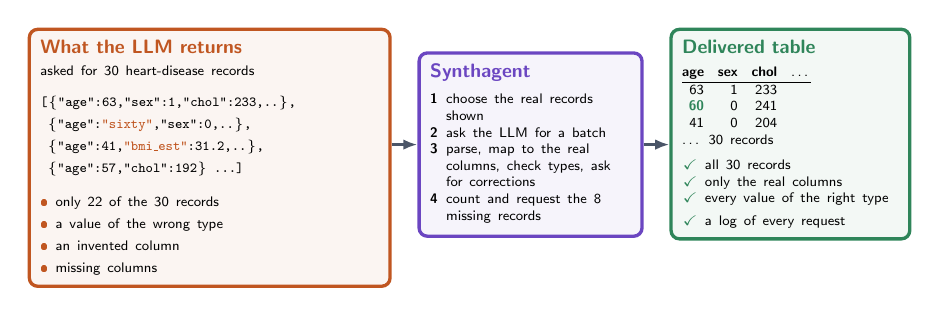
\begin{tikzpicture}[
  font=\sffamily\scriptsize,
  >={Latex[length=1.8mm]},
  box/.style={rounded corners=3pt,draw=#1,very thick,fill=#1!6,inner sep=4pt,align=left},
]
\providecommand{\bad}[1]{\textcolor{sorange}{\textbf{#1}}}
% ---------------- LLM response ----------------
\node[box=sorange,anchor=north west,text width=4.3cm] (raw) at (0,0) {%
  \textbf{\textcolor{sorange}{What the LLM returns}}\\
  {\tiny asked for 30 heart-disease records}\\[3pt]
  \texttt{\tiny [\{"age":63,"sex":1,"chol":233,..\},}\\
  \texttt{\tiny \ \{"age":\bad{"sixty"},"sex":0,..\},}\\
  \texttt{\tiny \ \{"age":41,\bad{"bmi\_est"}:31.2,..\},}\\
  \texttt{\tiny \ \{"age":57,"chol":192\} ...]}\\[4pt]
  {\tiny\bad{\textbullet} only 22 of the 30 records}\\
  {\tiny\bad{\textbullet} a value of the wrong type}\\
  {\tiny\bad{\textbullet} an invented column}\\
  {\tiny\bad{\textbullet} missing columns}};

% ---------------- Synthagent ----------------
\node[box=spurple,anchor=north west,text width=2.55cm] (ctl) at (4.95,-0.3) {%
  \textbf{\textcolor{spurple}{\system}}\\[3pt]
  {\tiny\setlength{\tabcolsep}{0pt}%
   \begin{tabular}{@{}l@{\hspace{3pt}}p{2.3cm}@{}}
   \textbf{1} & choose the real records shown\\
   \textbf{2} & ask the LLM for a batch\\
   \textbf{3} & parse, map to the real columns, check types, ask for corrections\\
   \textbf{4} & count and request the 8 missing records\\
   \end{tabular}}};

% ---------------- delivered table ----------------
\node[box=sgreen,anchor=north west,text width=2.75cm] (ok) at (8.15,0) {%
  \textbf{\textcolor{sgreen}{Delivered table}}\\[3pt]
  {\tiny\setlength{\tabcolsep}{2.5pt}%
   \begin{tabular}{@{}rrrc@{}}
   \textbf{age} & \textbf{sex} & \textbf{chol} & \dots\\\hline
   63 & 1 & 233 & \\
   \textcolor{sgreen}{\textbf{60}} & 0 & 241 & \\
   41 & 0 & 204 & \\
   \multicolumn{4}{@{}l}{\dots\ 30 records}\\
   \end{tabular}}\\[3pt]
  {\tiny\textcolor{sgreen}{\checkmark} all 30 records\\
   \textcolor{sgreen}{\checkmark} only the real columns\\
   \textcolor{sgreen}{\checkmark} every value of the right type\\
   \textcolor{sgreen}{\checkmark} a log of every request}};

\draw[->,very thick,sgray] (raw.east |- ctl.west) -- (ctl.west);
\draw[->,very thick,sgray] (ctl.east) -- (ok.west |- ctl.east);
\end{tikzpicture}
}
\caption{The problem addressed in this paper, in an illustrative example. Asked for 30 \DIFdelbeginFL \DIFdelFL{records of a }\DIFdelendFL heart-disease \DIFdelbeginFL \DIFdelFL{dataset}\DIFdelendFL \DIFaddbeginFL \DIFaddFL{records}\DIFaddendFL , \DIFdelbeginFL \DIFdelFL{an }\DIFdelendFL \DIFaddbeginFL \DIFaddFL{the }\DIFaddendFL LLM \DIFdelbeginFL \DIFdelFL{response }\DIFdelendFL (left) \DIFdelbeginFL \DIFdelFL{can contain }\DIFdelendFL \DIFaddbeginFL \DIFaddFL{returns }\DIFaddendFL too few records, \DIFaddbeginFL \DIFaddFL{an }\DIFaddendFL invented \DIFdelbeginFL \DIFdelFL{or }\DIFdelendFL \DIFaddbeginFL \DIFaddFL{column, }\DIFaddendFL missing \DIFdelbeginFL \DIFdelFL{features }\DIFdelendFL \DIFaddbeginFL \DIFaddFL{columns }\DIFaddendFL and \DIFdelbeginFL \DIFdelFL{values }\DIFdelendFL \DIFaddbeginFL \DIFaddFL{a value }\DIFaddendFL of the wrong type. \system (\DIFdelbeginFL \DIFdelFL{right}\DIFdelendFL \DIFaddbeginFL \DIFaddFL{middle}\DIFaddendFL ) \DIFdelbeginFL \DIFdelFL{validates }\DIFdelendFL \DIFaddbeginFL \DIFaddFL{checks }\DIFaddendFL and corrects every response \DIFaddbeginFL \DIFaddFL{and requests the missing records}\DIFaddendFL , \DIFdelbeginFL \DIFdelFL{so }\DIFdelendFL \DIFaddbeginFL \DIFaddFL{following }\DIFaddendFL the \DIFdelbeginFL \DIFdelFL{resulting dataset has no integrity violations}\DIFdelendFL \DIFaddbeginFL \DIFaddFL{four steps of Figure~\ref{fig:architecture}}\DIFaddendFL , and \DIFdelbeginFL \DIFdelFL{a log }\DIFdelendFL \DIFaddbeginFL \DIFaddFL{delivers all 30 }\DIFaddendFL records \DIFdelbeginFL \DIFdelFL{each correction }\DIFdelendFL \DIFaddbeginFL \DIFaddFL{with the columns }\DIFaddendFL and \DIFdelbeginFL \DIFdelFL{its cost}\DIFdelendFL \DIFaddbeginFL \DIFaddFL{types of the real data (right)}\DIFaddendFL .}
\label{fig:teaser}
\end{figure}

%======================================================================
\section{Background Knowledge}
\label{sec:related}
%======================================================================
\DIFdelbegin \DIFdel{This }\DIFdelend \DIFaddbegin \DIFadd{To place the problem of Section~\ref{sec:intro} in context, this }\DIFaddend section reviews the families of tabular SDG methods, their limitations when data are small, and the work on validating generated data and evaluating synthetic data on which \system builds.

\begin{table*}[!t]
\centering
\caption{Families of tabular SDG methods: how they produce records, their main limitation in small data, and their properties. \checkmark: provided by design; $\times$: not provided. SMOTE's number of records is set by the class balance, not by the user; fine-tuned language models discard unreadable records but do not check types; constrained decoding is a variant of prompted LLMs.}
\label{tab:positioning}
\footnotesize
\setlength{\tabcolsep}{3pt}
\begin{tabular}{@{}p{.15\textwidth}p{.23\textwidth}p{.27\textwidth}cccc@{}}
\toprule
Family & How records are produced & Main limitation in small data & \begin{tabular}[c]{@{}c@{}}No training on\\target data\end{tabular} & \begin{tabular}[c]{@{}c@{}}Record\\count\end{tabular} & \begin{tabular}[c]{@{}c@{}}Columns and\\types checked\end{tabular} & \begin{tabular}[c]{@{}c@{}}Cost\\recorded\end{tabular} \\
\midrule
Interpolation and statistical~\cite{chawla2002smote,zhang2014privbayes} & Combine real records or sample a simple model fitted to them & Only recombine existing patterns; ignore feature meaning & \checkmark & $\times$ & $\times$ & $\times$ \\
Deep generative~\cite{xu2019ctgan,kotelnikov2023tabddpm,zhang2024tabsyn} & Train a neural network on the real records and sample from it & Few records to fit many parameters; invalid or copied records & $\times$ & \checkmark & $\times$ & $\times$ \\
Fine-tuned language models~\cite{borisov2023great,solatorio2023realtabformer} & Fine-tune a language model on records written as text & Training on scarce records & $\times$ & \checkmark & $\times$ & $\times$ \\
Prompted LLMs~\cite{seedat2024cllm,kim2024epic} & Ask a pre-trained LLM for records, with real examples in the prompt & Unreliable output: missing or malformed records, unknown cost & \checkmark & $\times$ & $\times$ & $\times$ \\
Prompted LLMs, constrained decoding~\cite{willard2023outlines,geng2023grammar} & As above, with the output restricted to a JSON schema & Format guaranteed, but not the number of records; cost unknown & \checkmark & $\times$ & \checkmark & $\times$ \\
\midrule
\system (ours) & Prompted LLM whose output is checked and completed by a control layer & - & \checkmark & \checkmark & \checkmark & \checkmark \\
\bottomrule
\end{tabular}
\end{table*}

\subsection{Synthetic Data Generation for Tabular Data}
Tabular SDG methods fall into four families that differ in how they produce records. \emph{Interpolation and statistical methods} derive new records directly from the real ones or from a simple probabilistic model of them: SMOTE places a new minority-class record on the line segment between two neighbouring records of that class~\cite{chawla2002smote}, and Bayesian networks estimate the dependencies between features and sample new records from them~\cite{zhang2014privbayes,cai2021privmrf}. \emph{Deep generative models} train a neural network to approximate the joint distribution of the features and sample from it: CTGAN trains a generator against a discriminator, TVAE learns a compressed representation of the records~\cite{xu2019ctgan}, and diffusion models such as TabDDPM, CoDi and TabSyn learn to reverse a gradual corruption of the records~\cite{kotelnikov2023tabddpm,lee2023codi,zhang2024tabsyn}; relational and cross-silo variants extend these models to several tables or institutions~\cite{fan2020relational,shankar2024silofuse}. \emph{Fine-tuned language models} write each record as a sentence, fine-tune a language model on these sentences and generate new ones, as in GReaT~\cite{borisov2023great}, REaLTabFormer~\cite{solatorio2023realtabformer} and TabLoft~\cite{chen2026tabloft}. \emph{Prompted LLMs} place a few real records in the prompt of a pre-trained LLM and ask it for new ones, without training, as in CLLM~\cite{seedat2024cllm} and EPIC~\cite{kim2024epic}.

\subsection{Synthetic Data Generation in Small Data}
Most of these generators were designed and benchmarked on datasets with tens or hundreds of thousands of records, such as Adult (48,842 records) or Covertype (581,012 records)~\cite{xu2019ctgan}, and their behaviour on a few hundred records is far less studied. Table~\ref{tab:positioning} summarizes, for each family, how records are produced and its main limitation when data are small. Interpolation and statistical methods, as well as deep generators, are fitted only to the real records, so they cannot add information beyond what those records contain~\cite[Sec.~2.8]{cover2006elements}. They also treat every column as an anonymous number, ignoring what is known about variables such as age or cholesterol. Deep generators and fine-tuned language models have many parameters, which a few hundred records cannot estimate reliably, so they may produce records outside the observed ranges and types, or reproduce training records~\cite{hyeong2022tabularmia}. Prompted LLMs need no training and bring domain knowledge, but nothing ensures that their output contains the \DIFdelbegin \DIFdel{configured }\DIFdelend \DIFaddbegin \DIFadd{requested }\DIFaddend number of records with the correct columns and types, and the cost of obtaining it is not reported; CLLM~\cite{seedat2024cllm} filters the generated records by their learning dynamics and EPIC~\cite{kim2024epic} designs balanced prompts, but both concern the quality of the kept records rather than the integrity and cost of the output. \system keeps the advantages of prompted LLMs and adds the control layer that they lack.

\subsection{Validation of Generated Data}
The control layer applies to generation a principle long used in data management: data produced by an automatic process are checked against explicit constraints before they are accepted. Kamino enforces integrity constraints during private data synthesis~\cite{ge2021kamino}, data-cleaning systems combine statistical inference with integrity constraints~\cite{chu2013holistic,qin2024bclean}, and recovering structured records from the free-form output of an LLM has been studied as a data-engineering problem~\cite{rorseth2026recovering}, as have LLMs for data wrangling, error detection and document processing, which must cope with unreliable model output~\cite{narayan2022wrangle,ni2025zeroed,shankar2025docetl}. Constrained decoding restricts the tokens an LLM may emit to a grammar or JSON schema~\cite{willard2023outlines,geng2023grammar}, now offered by providers as a structured-output mode; it fixes the format of each response but not the number of records (Section~\ref{sec:rq1}). In \system, the constraints are the columns and types inferred from the real data, and every LLM response is checked, in the action-observation loop of LLM agents~\cite{yao2023react,wang2024agentsurvey}.

\subsection{Evaluating Synthetic Data}
Data-preparation studies have shown that a step that looks beneficial can harm downstream models~\cite{li2021cleanml,guha2023cleaningfairness}, and evaluation frameworks such as Synthcity and SynthEval recommend assessing fidelity, privacy and utility together~\cite{qian2023synthcity,lautrup2025syntheval}. Fidelity can be complemented by a classifier two-sample test, which asks whether a classifier can tell real from synthetic records~\cite{lopezpaz2017c2st}, and privacy by membership-inference attacks, which ask whether an attacker can tell which records were used for generation~\cite{shokri2017mia,hyeong2022tabularmia}. Formal guarantees require models such as $\ell$-diversity, $t$-closeness~\cite{machanavajjhala2006ldiversity,li2007tcloseness} or differential privacy~\cite{dwork2014dp}, which \system does not claim.

%======================================================================
\section{The \system System}
\label{sec:system}
%======================================================================
\DIFaddbegin \DIFadd{Section~\ref{sec:related} showed that no family both brings knowledge beyond the few real records and guarantees a usable dataset. }\DIFaddend \system \DIFdelbegin \DIFdel{meets the constraint }\DIFdelend \DIFaddbegin \DIFadd{does both. It meets the constraints }\DIFaddend of Equation~\eqref{eq:multiobjective}, a synthetic dataset with exactly $N$ records that conform to $S$, by construction rather than by trusting the LLM. \DIFdelbegin \DIFdel{This guarantee is the core of the system: the }\DIFdelend \DIFaddbegin \DIFadd{The }\DIFaddend LLM only proposes records; the control layer decides which to accept, asks for corrections or more records, and stops only when $N$ conforming records have been accepted or a stopping limit is reached. The objectives of Equation~\eqref{eq:multiobjective} are left to the LLM's domain knowledge and the real records shown to it; they are measured, not optimized, in Section~\ref{sec:results}. The real dataset is never modified.

Figure~\ref{fig:architecture} shows the architecture and Algorithm~\ref{alg:loop} the procedure. A profiling step first infers the columns and their types $S$ from the training records. Each request then passes through four stages: the context budgeter selects the real records shown to the LLM (1), the LLM proposes a batch of records (2), the deterministic verifier parses, maps and validates it (3), and the \DIFdelbegin \DIFdel{admitted }\DIFdelend \DIFaddbegin \DIFadd{accepted }\DIFaddend records are counted against $N$ (4). The run produces two outputs: the synthetic table $G$ and an audit trail of every request. The rest of this section follows this order and ends with the parameters and the reason for each value.

\begin{figure*}[t]
\centering
\resizebox{\textwidth}{!}{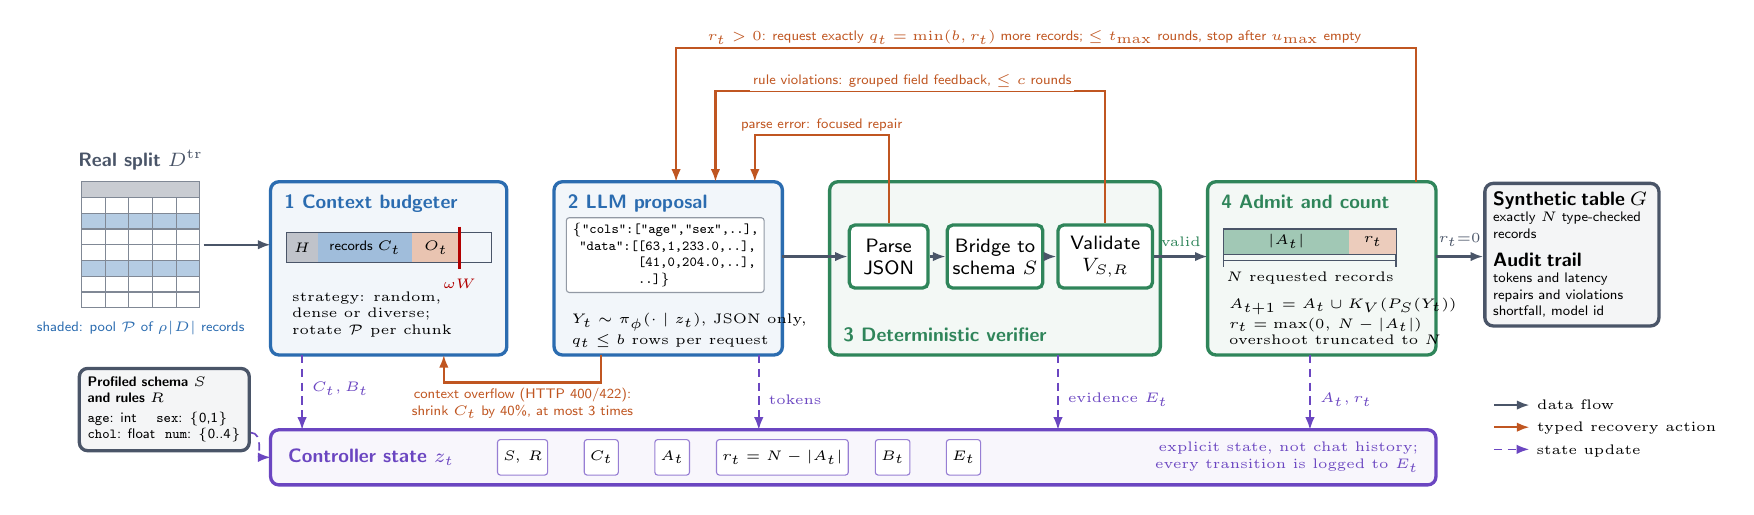
\begin{tikzpicture}[
  font=\sffamily\scriptsize,
  >={Latex[length=1.6mm]},
  flow/.style={->,thick,sgray},
  fail/.style={->,thick,sorange},
  st/.style={->,densely dashed,spurple,semithick},
  pan/.style={rounded corners=3pt,draw=#1,very thick,fill=#1!6},
  ttl/.style={font=\sffamily\bfseries\scriptsize,text=#1,anchor=north west},
  gate/.style={draw=sgreen,very thick,fill=white,rounded corners=2pt,minimum height=8mm,align=center,inner sep=2pt},
  lab/.style={font=\sffamily\tiny,text=#1,fill=white,inner sep=1pt},
]
%======================== panels ========================
\draw[pan=sblue]   (2.4,0) rectangle (5.4,-2.2);   \node[ttl=sblue]  at (2.45,-0.05) {1\,\,Context budgeter};
\draw[pan=sblue]   (6.0,0) rectangle (8.9,-2.2);   \node[ttl=sblue]  at (6.05,-0.05) {2\,\,LLM proposal};
\draw[pan=sgreen]  (9.5,0) rectangle (13.7,-2.2);  \node[ttl=sgreen,anchor=south west] at (9.55,-2.15) {3\,\,Deterministic verifier};
\draw[pan=sgreen]  (14.3,0) rectangle (17.2,-2.2); \node[ttl=sgreen] at (14.35,-0.05) {4\,\,Admit and count};

%======================== real data =====================
\foreach \r in {1,...,7}{\foreach \c in {0,...,4}{
   \ifnum\r=2 \fill[sblue!35] (\c*0.3,-\r*0.2) rectangle ++(0.3,-0.2);\fi
   \ifnum\r=5 \fill[sblue!35] (\c*0.3,-\r*0.2) rectangle ++(0.3,-0.2);\fi
   \draw[sgray!70] (\c*0.3,-\r*0.2) rectangle ++(0.3,-0.2);}}
\fill[sgray!30] (0,0) rectangle (1.5,-0.2); \draw[sgray!70] (0,0) rectangle (1.5,-0.2);
\node[font=\sffamily\bfseries\scriptsize,text=sgray,anchor=south] at (0.75,0.02) {Real split $D^{\mathrm{tr}}$};
\node[font=\sffamily\tiny,text=sblue,align=center,anchor=north] at (0.75,-1.65) {shaded: pool $\mathcal{P}$ of $\rho|D|$ records};
\draw[flow] (1.55,-0.8) -- (2.4,-0.8);

% profile card
\node[pan=sgray,anchor=north west,align=left,inner sep=3pt,font=\sffamily\tiny] (prof) at (-0.05,-2.35)
  {\textbf{Profiled schema $S$}\\\textbf{and rules $R$}\\[1pt]
   \texttt{age}: int \quad \texttt{sex}: \{0,1\}\\ \texttt{chol}: float \ \texttt{num}: \{0..4\}};

%======================== 1 budgeter ====================
\begin{scope}[shift={(2.6,-0.65)}]
  \fill[sgray!35]   (0,0) rectangle (0.4,-0.38);  \node at (0.2,-0.19)  {\tiny $H$};
  \fill[sblue!45]   (0.4,0) rectangle (1.6,-0.38); \node at (1.0,-0.19) {\tiny records $C_t$};
  \fill[sorange!35] (1.6,0) rectangle (2.2,-0.38); \node at (1.9,-0.19) {\tiny $O_t$};
  \draw[sgray] (0,0) rectangle (2.6,-0.38);
  \draw[red!70!black,thick] (2.2,0.08) -- (2.2,-0.46);
  \node[font=\tiny,text=red!70!black,anchor=north] at (2.2,-0.46) {$\omega W$};
  \node[font=\tiny,anchor=north west,align=left] at (-0.05,-0.62)
     {strategy: random,\\dense or diverse;\\rotate $\mathcal{P}$ per chunk};
\end{scope}

%======================== 2 LLM =========================
\node[anchor=north west,draw=sgray!60,fill=white,rounded corners=1pt,align=left,font=\ttfamily\tiny,inner sep=2pt]
  at (6.15,-0.45)
  {\{"cols":["age","sex",..],\\ \ "data":[[63,1,233.0,..],\\ \hphantom{\ "data":[}[41,0,204.0,..],\\ \hphantom{\ "data":[}..]\}};
\node[font=\tiny,anchor=north west,align=left] at (6.1,-1.55) {$Y_t\sim\pi_\phi(\cdot\mid z_t)$, JSON only,\\ $q_t\le b$ rows per request};

%======================== 3 verifier ====================
\node[gate,minimum width=10mm] (g1) at (10.25,-0.95) {Parse\\JSON};
\node[gate,minimum width=12mm] (g2) at (11.6,-0.95)  {Bridge to\\schema $S$};
\node[gate,minimum width=12mm] (g3) at (13.0,-0.95)  {Validate\\$V_{S,R}$};
\draw[flow] (g1)--(g2); \draw[flow] (g2)--(g3);
\draw[flow] (8.9,-0.95) -- (g1.west);

%======================== 4 admit =======================
\begin{scope}[shift={(14.5,-0.6)}]
  \fill[sgreen!45]  (0,0) rectangle (1.6,-0.32);
  \fill[sorange!30] (1.6,0) rectangle (2.2,-0.32);
  \draw[sgray] (0,0) rectangle (2.2,-0.32);
  \node at (0.8,-0.16) {\tiny $|A_t|$}; \node at (1.9,-0.16) {\tiny $r_t$};
  \draw[sgray,|-|] (0,-0.4) -- (2.2,-0.4);
  \node[font=\tiny,anchor=north] at (1.1,-0.42) {$N$ requested records};
  \node[font=\tiny,anchor=north west,align=left] at (-0.05,-0.75)
    {$A_{t+1}=A_t\cup K_V(P_S(Y_t))$\\$r_t=\max(0,\,N-|A_t|)$\\overshoot truncated to $N$};
\end{scope}
\draw[flow] (g3.east) -- node[above,font=\tiny,text=sgreen]{valid} (14.3,-0.95);

%======================== output ========================
\node[pan=sgray,anchor=north west,align=left,inner sep=3pt,text width=20mm,font=\sffamily\tiny] (out) at (17.8,0)
  {\textbf{\scriptsize Synthetic table $G$}\\exactly $N$ type-checked records\\[4pt]\textbf{\scriptsize Audit trail}\\tokens and latency\\repairs and violations\\shortfall, model id};
\draw[flow] (17.2,-0.95) -- node[above,font=\tiny]{$r_t{=}0$} (out.west|-0,-0.95);

%======================== recovery loops ================
% parse error -> focused repair
\draw[fail] (g1.north) -- (10.25,0.6) -- (8.55,0.6) -- (8.55,0);
\node[lab=sorange,anchor=south] at (9.4,0.6) {parse error: focused repair};
% violations -> grouped feedback
\draw[fail] (g3.north) -- (13.0,1.15) -- (8.05,1.15) -- (8.05,0);
\node[lab=sorange,anchor=south] at (10.55,1.15) {rule violations: grouped field feedback, $\le c$ rounds};
% residual -> top-up
\draw[fail] (16.95,0) -- (16.95,1.7) -- (7.55,1.7) -- (7.55,0);
\node[lab=sorange,anchor=south] at (12.1,1.7) {$r_t>0$: request exactly $q_t=\min(b,r_t)$ more records; $\le t_{\max}$ rounds, stop after $u_{\max}$ empty};
% overflow -> shrink context (below)
\draw[fail] (6.6,-2.2) -- (6.6,-2.55) -- (4.6,-2.55) -- (4.6,-2.2);
\node[lab=sorange,anchor=north,align=center] at (5.6,-2.58) {context overflow (HTTP 400/422):\\shrink $C_t$ by 40\%, at most 3 times};

%======================== state register ================
\draw[draw=spurple,very thick,fill=spurple!5,rounded corners=3pt] (2.4,-3.15) rectangle (17.2,-3.85);
\node[font=\sffamily\bfseries\scriptsize,text=spurple,anchor=west] at (2.5,-3.5) {Controller state $z_t$};
\foreach \lab/\x in {{$S,\,R$}/5.6,{$C_t$}/6.6,{$A_t$}/7.5,{$r_t=N-|A_t|$}/8.9,{$B_t$}/10.3,{$E_t$}/11.2}{
  \node[draw=spurple!70,fill=white,rounded corners=1pt,minimum height=4.5mm,inner sep=2pt,font=\tiny] at (\x,-3.5) {\lab};}
\node[font=\tiny,text=spurple,anchor=east,align=right] at (17.1,-3.5) {explicit state, not chat history;\\every transition is logged to $E_t$};
\draw[st] (prof.south east) ++(0,0.25) to[out=0,in=180] (2.4,-3.5);
\draw[st] (2.8,-2.2) -- (2.8,-3.15) node[pos=.45,right,font=\tiny]{$C_t,B_t$};
\draw[st] (8.6,-2.2) -- (8.6,-3.15) node[pos=.6,right,font=\tiny]{tokens};
\draw[st] (12.4,-2.2) -- (12.4,-3.15) node[pos=.6,right,font=\tiny]{evidence $E_t$};
\draw[st] (15.6,-2.2) -- (15.6,-3.15) node[pos=.6,right,font=\tiny]{$A_t,r_t$};

%======================== legend ========================
\node[anchor=north west,font=\tiny,align=left] at (17.8,-2.65) {
  \tikz\draw[flow](0,0)--(0.45,0); data flow\\[2pt]
  \tikz\draw[fail](0,0)--(0.45,0); typed recovery action\\[2pt]
  \tikz\draw[st](0,0)--(0.45,0); state update};
\end{tikzpicture}
}
\caption{Architecture of \system. The context budgeter selects the real records shown to the LLM (1); the LLM proposes a batch of records (2); the deterministic verifier parses it, maps it to the columns and types $S$ and validates it (3); and the \DIFdelbeginFL \DIFdelFL{admitted }\DIFdelendFL \DIFaddbeginFL \DIFaddFL{accepted }\DIFaddendFL records are counted against the \DIFdelbeginFL \DIFdelFL{configured }\DIFdelendFL \DIFaddbeginFL \DIFaddFL{requested }\DIFaddendFL number $N$ (4). Each failure type triggers its own correction (orange). Every stage reads or updates the controller state $z_t$ (purple). The outputs are the synthetic table $G$ and the audit trail of the run.}
\label{fig:architecture}
\end{figure*}

\begin{algorithm}[t]
\caption{Generation procedure of \system}
\label{alg:loop}
\small
\DIFdelbegin %DIFDELCMD < \begin{algorithmic}[1]
%DIFDELCMD < \Require training records $D$, columns and types $S$, number of records $N$, parameters of Table~\ref{tab:params}
%DIFDELCMD < \State pool $\mathcal{P}\gets$ random sample of $\rho|D|$ records of $D$
%DIFDELCMD < \State accepted records $A\gets\emptyset$ \Comment{empty at the start}
%DIFDELCMD < \Repeat
%DIFDELCMD <   \State context $C\gets$ next records of $\mathcal{P}$ that fit in a share $\omega$ of the context window $W$ \Comment{(1)}
%DIFDELCMD <   \State batch $Y\gets$ ask the LLM for $\min(b,N-|A|)$ new records, given $S$ and $C$ \Comment{(2)}
%DIFDELCMD <   \State records $X\gets$ parse the batch $Y$, repairing it if needed, and map its columns to $S$ \Comment{(3)}
%DIFDELCMD <   \State correct the invalid values of $X$, for at most $c$ rounds \Comment{(3)}
%DIFDELCMD <   \State $A\gets A\cup X$; log tokens, repairs and violations \Comment{(4)}
%DIFDELCMD < \Until{$|A|\ge N$ \textbf{or} $t_{\max}$ rounds \textbf{or} $u_{\max}$ empty answers}
%DIFDELCMD < \State \Return synthetic table $G$, the first $N$ records of $A$, and the audit trail
%DIFDELCMD < \end{algorithmic}
%DIFDELCMD < %%%
\DIFdelend \DIFaddbegin \begin{algorithmic}[1]
\Require training records $D$, columns and types $S$, number of records $N$, parameters of Table~\ref{tab:params}
\State pool $\mathcal{P}\gets$ random sample of $\rho|D|$ records of $D$
\State accepted records $A\gets\emptyset$ 
\Repeat
  \State context $C\gets$ next records of $\mathcal{P}$ that fit in a share $\omega$ of the context window $W$ \Comment{(1)}
  \State batch $Y\gets$ ask the LLM for $\min(b,N-|A|)$ new records, given $S$ and $C$ \Comment{(2)}
  \State records $X\gets$ parse the batch $Y$, repairing it if needed, and map its columns to $S$ \Comment{(3)}
  \State correct the invalid values of $X$, for at most $c$ rounds \Comment{(3)}
  \State $A\gets A\cup X$; log tokens, repairs and violations \Comment{(4)}
\Until{$|A|\ge N$ \textbf{or} $t_{\max}$ rounds \textbf{or} $u_{\max}$ empty answers}
\State \Return synthetic table $G$, the first $N$ records of $A$, and the audit trail
\end{algorithmic}
\DIFaddend \end{algorithm}

\subsection{Controller State}
\DIFaddbegin \DIFadd{The four stages share one state, the register at the bottom of Figure~\ref{fig:architecture}, which each stage reads and updates. }\DIFaddend At every step $t$, the control layer keeps
\DIFdelbegin \DIFdel{an explicit state
}\DIFdelend \begin{equation}
z_t=(S,\,C_t,\,A_t,\,N-|A_t|,\,B_t,\,E_t),
\label{eq:state}
\end{equation}
made of the columns and types $S$, the real records $C_t$ currently shown to the LLM, the synthetic records $A_t$ accepted so far, the number of records still missing $N-|A_t|$, the number of tokens $B_t$ still available in the context window, and the log $E_t$ of parser and validator results. From this state the LLM, denoted $\pi_{\phi}$, proposes a batch $Y_t\sim\pi_{\phi}(\cdot\mid z_t)$, and the accepted set grows only through the verifier:
\begin{equation}
A_{t+1}=A_t\cup \DIFdelbegin \DIFdel{K}\DIFdelend \DIFaddbegin \DIFadd{\Gamma}\DIFaddend \bigl(V_S\bigl(P_S(Y_t)\bigr)\bigr),
\label{eq:acceptance}
\end{equation}
where $P_S$ parses the batch $Y_t$ and maps its columns to $S$, $V_S$ validates the types, and \DIFdelbegin \DIFdel{$K$ sends the }\DIFdelend \DIFaddbegin \DIFadd{$\Gamma$ returns the records after sending their }\DIFaddend invalid values back to the LLM for correction\DIFaddbegin \DIFadd{, in at most $c$ rounds}\DIFaddend . Because the state is explicit rather than implied by the conversation history, the number of missing records is always known, and the parser log $E_t$ records every failure for later inspection.

\subsection{Context Budgeter (1)}
\DIFdelbegin \DIFdel{The context budgeter }\DIFdelend \DIFaddbegin \DIFadd{Each request starts with the context budgeter (stage 1; line 4 of Algorithm~\ref{alg:loop}), which }\DIFaddend decides which real records the LLM sees \DIFaddbegin \DIFadd{and sets $C_t$ and $B_t$ in the state}\DIFaddend . It draws a random sample of $\rho|D|$ training records, between \DIFdelbegin \DIFdel{31 and 123 }\DIFdelend \DIFaddbegin \DIFadd{18 and 122 }\DIFaddend records in our datasets, written as compact JSON with the feature columns and the class, so that the model sees how features and class co-occur. Because a long prompt can exceed the context window $W$ of the LLM, each request shows as many records of the sample as fit in a share $\omega$ of the window:
\begin{equation}
\begin{aligned}
C_t&=\operatorname{Slice}_{t}\bigl(\operatorname{Select}_{s}(D,\lceil\rho|D|\rceil),k_t\bigr),\\
k_t&=\max\{k:T(C_{t,k})\leq\omega W\},
\end{aligned}
\label{eq:context}
\end{equation}
where $\operatorname{Select}_s$ draws the sample with strategy $s$, \DIFaddbegin \DIFadd{$C_{t,k}$ are the first $k$ records of that slice, }\DIFaddend $T$ estimates the length in tokens of a prompt with \DIFdelbegin \DIFdel{$k$ records}\DIFdelend \DIFaddbegin \DIFadd{them}\DIFaddend , and $\operatorname{Slice}_t$ rotates through the sample, so that successive requests see different patients. If the provider still rejects a request as too long, the budgeter shows fewer records and retries. Besides the default random strategy, \emph{dense} prefers records with fewer missing values, and \emph{diverse} selects the records closest to the centres of $k$-means clusters. Neither strategy is class-stratified, a limitation discussed in Section~\ref{sec:discussion}.

\subsection{LLM Proposal and Prompts (2)}
\DIFdelbegin \DIFdel{The LLM }\DIFdelend \DIFaddbegin \DIFadd{With these records, the LLM is asked for a batch $Y_t$ (stage 2; line 5). It }\DIFaddend receives the same \DIFdelbegin \DIFdel{three-part }\DIFdelend conversation for every dataset and LLM (Table~\ref{tab:prompt-context}). A first message gives the column names and the sampled records in a compact format, a list of column names followed by one list of values per record. A generation message then asks for an exact number of new records, at most $b$, and states an output contract: JSON only, the same columns in the same order, a value in every cell, raw numbers, and no additional columns. No free-text description of the dataset or of the prediction task is added, so that no dataset receives more prompt engineering than another. The prompts are therefore deliberately simple, and their wording is not part of the contribution: the guarantees come from the stages that check the response.

\begin{table*}[t]
\centering
\caption{What the LLM receives in one generation request. The prompts are the same for every dataset and LLM. ``Not supplied'' is intentional: those signals cannot influence the generated records.}
\label{tab:prompt-context}
\footnotesize
\begin{tabular}{p{.17\textwidth}p{.36\textwidth}p{.39\textwidth}}
\toprule
Context layer & What the model receives & Why it is included or excluded \\
\midrule
Schema & Ordered column names and an exact column-count requirement & Fixes the record interface and prevents invented or omitted fields. \\
Demonstrations & Compact row-major serialization of a sample of $\rho|D|$ training records, with feature and target values & Exposes joint patterns, value formats, label prevalence and plausible cross-column combinations without sending the whole local table. \\
Generation task & Exact number of new records for the current batch, at most $b$ & Turns an open-ended completion into a bounded action whose output count can be verified. \\
Output contract & JSON only, fixed column order, complete cells, raw numeric values, no extra metadata & Makes parsing deterministic and removes interface failures unrelated to statistical quality. \\
Dynamic feedback & Parser error location after malformed JSON, or grouped field violations after failed validation & Reveals only the evidence needed for a targeted repair instead of replaying the full history. \\
Free-text metadata & Not supplied & Prevents unequal, dataset-specific prompt engineering from confounding the comparison. \\
Test information & No holdout rows, predictions, metrics or classifier identities & Preserves the evaluation boundary and prevents optimization against the test set. \\
Global statistics & No separately computed means, quantiles, correlations or class quotas & Fidelity must arise from the selected records; the consequence is weaker protection against rare-mode omission. \\
\bottomrule
\end{tabular}
\end{table*}

\subsection{Deterministic Verifier (3)}
The \DIFdelbegin \DIFdel{verifier turns a response }\DIFdelend \DIFaddbegin \DIFadd{batch $Y_t$ is text, not yet data. The verifier (stage 3; lines 6-7) turns it }\DIFaddend into records that conform to $S$, in three steps\DIFaddbegin \DIFadd{, and writes every failure to $E_t$}\DIFaddend . \emph{Parsing} extracts the records with a local parser that removes surrounding text and code fences, deletes trailing commas, inserts missing commas between records and closes a response truncated by the output limit. If parsing still fails, the control layer sends one repair request that quotes the position and the text around the error, at a low temperature so that the repair fixes the syntax without changing the content. \emph{Mapping} assigns the returned values to the columns of $S$: by position when the response has the expected number of columns, and otherwise by matching the returned column names to those of $S$, ignoring case and spacing; an invented column is dropped and a missing one is left empty. \emph{Validation} checks every value against the type that profiling inferred for its column (integer, real or categorical); optional rules can also bound numerical ranges or restrict categories, but they were off in our experiments except in the range-enforcement variant. The invalid values are grouped by column and sent back to the LLM with one example per column, for at most $c$ correction rounds, so that the model corrects only what is wrong instead of regenerating the batch. The three steps escalate from cheap to costly: a defect that the local parser or the mapping can fix costs no request, a syntax error costs one repair request, and only type violations cost correction rounds. In the example of Figure~\ref{fig:teaser}, the parser recovers the 22 records, the mapping drops the invented column \texttt{bmi\_est} and leaves the missing columns empty, the validator flags \texttt{age="sixty"}, and one correction round replaces it with a number; the completion loop then requests the eight missing records. Every step is written to the parser log $E_t$.

\subsection{Admit and Count (4)}
\DIFaddbegin \DIFadd{Only the records that pass the verifier reach the last stage (stage 4; line 8), which adds them to $A_t$ and decides whether to ask for more. }\DIFaddend LLMs often return fewer records than requested\DIFdelbegin \DIFdel{. The admitted }\DIFdelend \DIFaddbegin \DIFadd{, so the accepted }\DIFaddend records are counted against $N$, and after the planned batches the completion loop requests only the missing records,
\begin{equation}
r_t=\max(0,N-|A_t|),\qquad q_t=\min(b,r_t),
\label{eq:residual}
\end{equation}
\DIFdelbegin \DIFdel{and }\DIFdelend \DIFaddbegin \DIFadd{where $r_t$ is the number of records still missing and $q_t$ the number requested in round $t$, at most the batch size $b$; the loop also }\DIFaddend truncates any excess. It stops when $N$ records have been accepted, after $t_{\max}$ rounds, or after $u_{\max}$ consecutive empty answers; a run that ends short because the provider keeps failing is recorded as such. The run returns the synthetic table $G$ and an audit trail with the tokens processed, the generation time, the repairs, the violations and the requested and delivered numbers of records, which makes a synthetic dataset inspectable after the fact and gives the cost $\kappa$ in Equation~\eqref{eq:multiobjective} a measured value.

\subsection{Parameters}
\DIFaddbegin \DIFadd{The parameters introduced with each stage are collected in }\DIFaddend Table~\ref{tab:params} \DIFdelbegin \DIFdel{lists the parameters and }\DIFdelend \DIFaddbegin \DIFadd{with }\DIFaddend the values used in the experiments, fixed beforehand from the size of our datasets and the context and output limits of the LLMs rather than tuned on the results; Section~\ref{sec:rq1} examines their effect.

\begin{table}[t]
\centering
\caption{Parameters of the control layer, the values used in the experiments and the reason for each value. The LLM-chosen settings variant (Section~\ref{sec:setup}) lets the LLM choose the first and fourth instead.}
\label{tab:params}
\footnotesize
\setlength{\tabcolsep}{2pt}
\DIFdelbeginFL %DIFDELCMD < \begin{tabular}{@{}p{.27\columnwidth}p{.15\columnwidth}p{.52\columnwidth}@{}}
%DIFDELCMD < \toprule
%DIFDELCMD < Parameter & Value & Reason \\
%DIFDELCMD < \midrule
%DIFDELCMD < Context sample $\rho$ & 20\% of training records & 31 to 123 records in our datasets: enough to show the main patterns of the data, while the prompt still fits the context window of every LLM tested \\
%DIFDELCMD < Window share $\omega$ & 85\% & Leaves room for the answer and for errors in the estimated prompt length \\
%DIFDELCMD < Batch size $b$ & 30 records & The longest answer (30 records of the 30-feature dataset) stays within the output limit of every LLM tested; a failed answer loses at most 30 records \\
%DIFDELCMD < Temperature & 0.3 & Favours adherence to the output format while keeping some diversity \\
%DIFDELCMD < Repair temperature & 0.1 & A repair should fix the syntax, not change the content \\
%DIFDELCMD < Correction rounds $c$ & 2 & Bounds the cost of a batch that keeps failing \\
%DIFDELCMD < Top-up rounds $t_{\max}$ & 50 & $50\times30=1{,}500$ records, more than twice the largest $N$ (614) \\
%DIFDELCMD < Empty-answer limit $u_{\max}$ & 5 & Five consecutive empty answers indicate a provider failure rather than a sampling accident \\
%DIFDELCMD < \bottomrule
%DIFDELCMD < \end{tabular}
%DIFDELCMD < %%%
\DIFdelendFL \DIFaddbeginFL \begin{tabular}{@{}>{\raggedright\arraybackslash}p{.27\columnwidth}>{\raggedright\arraybackslash}p{.15\columnwidth}>{\raggedright\arraybackslash}p{.52\columnwidth}@{}}
\toprule
Parameter & Value & Reason \\
\midrule
Context sample $\rho$ & 20\% of training records & 18 to 122 records in our datasets: enough to show the main patterns of the data, while the prompt still fits the context window of every LLM tested \\
Window share $\omega$ & 85\% & Leaves room for the answer and for errors in the estimated prompt length \\
Batch size $b$ & 30 records & The longest answer (30 records of the 30-feature dataset) stays within the output limit of every LLM tested; a failed answer loses at most 30 records \\
Temperature & 0.3 & Favours adherence to the output format while keeping some diversity \\
Repair temperature & 0.1 & A repair should fix the syntax, not change the content \\
Correction rounds $c$ & 2 & Bounds the cost of a batch that keeps failing \\
Completion rounds $t_{\max}$ & 50 & $50\times30=1{,}500$ records, more than twice the largest $N$ (614) \\
Empty-answer limit $u_{\max}$ & 5 & Five consecutive empty answers indicate a provider failure rather than a sampling accident \\
\bottomrule
\end{tabular}
\DIFaddendFL \end{table}

%======================================================================
\section{Deployment \DIFdelbegin \DIFdel{Across }\DIFdelend \DIFaddbegin \DIFadd{across }\DIFaddend Healthcare Facilities}
\label{sec:deployment}
%======================================================================
\DIFdelbegin \DIFdel{This section outlines a deployment design, which this paper does not evaluate}\DIFdelend \DIFaddbegin \DIFadd{Section~\ref{sec:system} described }\system \DIFadd{at one facility}\DIFaddend . Healthcare facilities\DIFaddbegin \DIFadd{, however, }\DIFaddend often cannot pool their records (Section~\ref{sec:intro})~\cite{rieke2020digitalhealth,sheller2020medicine}, \DIFdelbegin \DIFdel{and }\DIFdelend \DIFaddbegin \DIFadd{so this section outlines how }\DIFaddend \system \DIFdelbegin \DIFdel{was designed for this setting}\DIFdelend \DIFaddbegin \DIFadd{can serve several of them, a design this paper does not evaluate}\DIFaddend . Because the control layer needs only a local dataset, its \DIFdelbegin \DIFdel{schema }\DIFdelend \DIFaddbegin \DIFadd{columns and types }\DIFaddend and an inference endpoint, each facility of a network can run it inside its own infrastructure. Consider $K$ healthcare facilities, each holding a small dataset $D_k$ for the same prediction task, with different case mix, coding practice and class prevalence. Each facility runs \system locally and trains on its real and synthetic records,
\begin{equation}
G_k=\mathcal{A}(D_k,S_k,N_k),\qquad
\Delta w_k=\mathcal{U}(w\DIFdelbegin \DIFdel{_t}\DIFdelend \DIFaddbegin \DIFadd{_\tau}\DIFaddend ,D_k\cup G_k),
\label{eq:local-federated}
\end{equation}
where \DIFaddbegin \DIFadd{$\mathcal{A}$ denotes }\system\DIFadd{, }\DIFaddend $S_k$ are the local columns and types, $N_k$ the local number of synthetic records\DIFaddbegin \DIFadd{, $w_\tau$ the shared model at aggregation round $\tau$ }\DIFaddend and $\mathcal{U}$ the local training procedure. Only the model update $\Delta w_k$ and approved aggregate diagnostics leave the facility. A coordinator aggregates the updates as in FedAvg~\cite{mcmahan2017fedavg,kairouz2021federated},
\begin{equation}
w\DIFdelbegin \DIFdel{_{t+1}}\DIFdelend \DIFaddbegin \DIFadd{_{\tau+1}}\DIFaddend =w\DIFdelbegin \DIFdel{_t}\DIFdelend \DIFaddbegin \DIFadd{_\tau}\DIFaddend +\sum\DIFdelbegin \DIFdel{_{k\in\mathcal{K}_t}\frac{n_k}{\sum_{j\in\mathcal{K}_t}n_j}}\DIFdelend \DIFaddbegin \DIFadd{_{k\in\mathcal{K}_\tau}\frac{n_k}{\sum_{j\in\mathcal{K}_\tau}n_j}}\DIFaddend \,\Delta w_k,\qquad n_k=|D_k|,
\label{eq:federated-aggregate}
\end{equation}
\DIFaddbegin \DIFadd{where $\mathcal{K}_\tau$ is the set of facilities taking part in round $\tau$, }\DIFaddend preferably under secure aggregation~\cite{bonawitz2017secure}. The weights count \emph{real} records, $|D_k|$ rather than $|D_k\cup G_k|$, so a facility gains no extra weight by generating more records (Figure~\ref{fig:federated}). Unlike SiloFuse, which trains a shared generator across sites~\cite{shankar2024silofuse}, this design needs no generator training across facilities, and each facility can reject its synthetic records when paired local validation shows no gain. The design is not, by itself, a privacy guarantee: with a remote LLM the prompt content leaves the facility, so sensitive deployments need a locally served model or a data-processing agreement, and both synthetic records and model updates can leak information~\cite{chen2024modeltrip}. Our experiments evaluate the generation step one facility at a time, as the next section describes; a multi-facility evaluation is future work.



\DIFdelbegin %DIFDELCMD < \begin{figure*}[t]
%DIFDELCMD < %%%
\DIFdelendFL \DIFaddbeginFL \begin{figure}[t]
\DIFaddendFL \centering
\DIFdelbeginFL %DIFDELCMD < \begin{minipage}[c]{0.6\textwidth}
%DIFDELCMD < \resizebox{\linewidth}{!}{% Cross-silo deployment figure (Fig. fig:federated). Requires TikZ libraries
% arrows.meta, calc, shapes.geometric and the s* colours from main.tex.
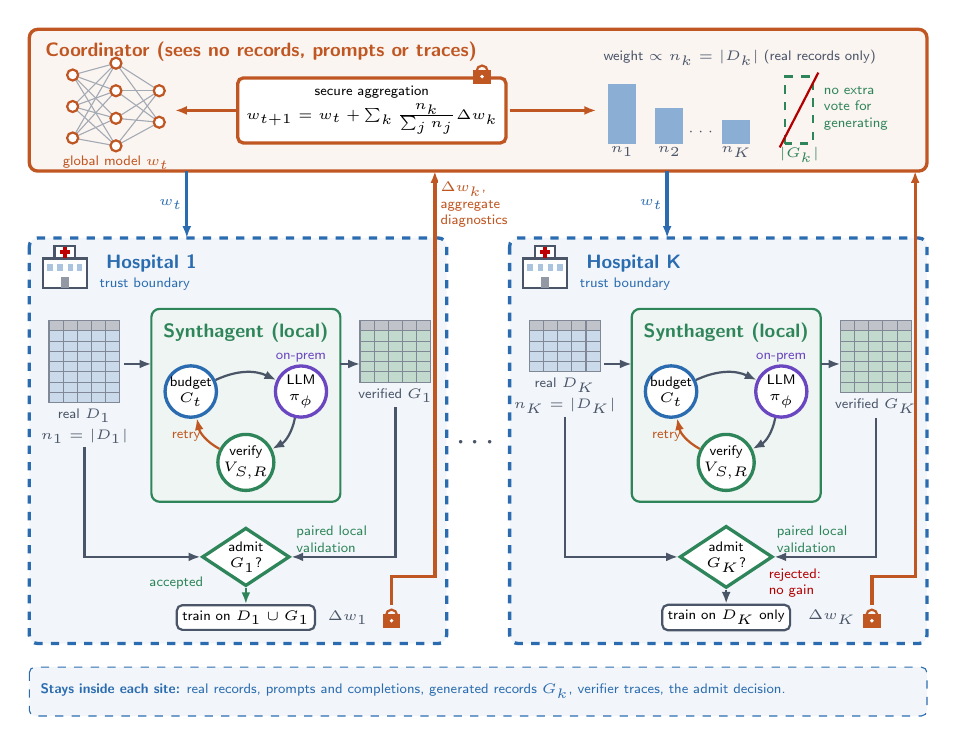
\begin{tikzpicture}[
  font=\sffamily\scriptsize,
  >={Latex[length=1.5mm]},
  flow/.style={->,thick,sgray},
  down/.style={->,very thick,sblue},
  up/.style={->,very thick,sorange},
  pan/.style={rounded corners=3pt,draw=#1,very thick,fill=#1!6},
  ttl/.style={font=\sffamily\bfseries\scriptsize,text=#1},
  lab/.style={font=\sffamily\tiny,text=#1,inner sep=1pt},
  nd/.style={circle,draw=#1,very thick,fill=white,minimum size=6.5mm,inner sep=0pt,font=\sffamily\tiny,align=center},
  diam/.style={diamond,aspect=1.5,draw=sgreen,very thick,fill=white,inner sep=0.5pt,font=\sffamily\tiny,align=center},
]
%---------------------------------------------------------------- icons
\def\lock#1#2{% padlock at (#1), colour #2
  \begin{scope}[shift={(#1)}]
    \draw[#2,thick] (-0.07,0.05) arc[start angle=180,end angle=0,radius=0.07];
    \fill[#2] (-0.11,-0.11) rectangle (0.11,0.06);
    \fill[white] (0,-0.02) circle (0.025);
  \end{scope}}
\def\hospital#1{% small hospital building at (#1)
  \begin{scope}[shift={(#1)}]
    \fill[white,draw=sgray,thick] (-0.28,-0.22) rectangle (0.28,0.16);
    \fill[white,draw=sgray,thick] (-0.13,0.16) rectangle (0.13,0.32);
    \fill[red!75!black] (-0.025,0.17) rectangle (0.025,0.31);
    \fill[red!75!black] (-0.065,0.215) rectangle (0.065,0.265);
    \foreach \x in {-0.19,-0.06,0.07,0.19}{\fill[sblue!40] (\x-0.035,0.0) rectangle ++(0.07,0.09);}
    \fill[sgray!60] (-0.05,-0.22) rectangle (0.05,-0.08);
  \end{scope}}
\def\tabl#1#2#3#4{% table glyph at (#1): #2 rows, row fill #3, highlighted row #4
  \begin{scope}[shift={(#1)}]
    \fill[sgray!35] (0,0) rectangle (0.9,-0.13);
    \foreach \r in {1,...,#2}{
      \ifnum\r=#4 \fill[sorange!45] (0,-0.13*\r) rectangle (0.9,-0.13*\r-0.13);
      \else \fill[#3] (0,-0.13*\r) rectangle (0.9,-0.13*\r-0.13);\fi}
    \foreach \c in {0,0.18,...,0.73}{\draw[sgray!70] (\c,0) rectangle ++(0.18,-0.13*#2-0.13);}
    \foreach \r in {0,...,#2}{\draw[sgray!70] (0,-0.13*\r) -- (0.9,-0.13*\r);}
  \end{scope}}
%---------------------------------------------------------------- one hospital site
% #1 x-offset, #2 site index label, #3 real rows (n_k), #4 generated rows,
% #5 admit decision text, #6 admit colour
\def\site#1#2#3#4#5#6{%
\begin{scope}[shift={(#1,0)}]
  % trust boundary
  \draw[pan=sblue,dashed] (0,0) rectangle (5.3,-5.15);
  \hospital{0.45,-0.42}
  \node[ttl=sblue,anchor=west] at (0.85,-0.32) {Hospital #2};
  \node[lab=sblue,anchor=west] at (0.85,-0.58) {trust boundary};
  % private data
  \tabl{0.25,-1.05}{#3}{sblue!25}{0}
  \node[lab=sgray,anchor=north] at (0.7,-1.05-0.13*#3-0.17) {real $D_#2$};
  \node[lab=sgray,anchor=north] at (0.7,-1.05-0.13*#3-0.42) {$n_#2=|D_#2|$};
  % local Synthagent loop
  \fill[sgreen!8,draw=sgreen,rounded corners=3pt,thick] (1.55,-0.9) rectangle (3.95,-3.35);
  \node[ttl=sgreen,anchor=north] at (2.75,-0.95) {\system{} (local)};
  \node[nd=sblue]  (b#2) at (2.05,-1.95) {budget\\$C_t$};
  \node[nd=spurple](l#2) at (3.45,-1.95) {LLM\\$\pi_\phi$};
  \node[nd=sgreen] (v#2) at (2.75,-2.85) {verify\\$V_{S,R}$};
  \draw[flow,bend left=25] (b#2) to (l#2);
  \draw[flow,bend left=25] (l#2) to (v#2);
  \draw[->,thick,sorange,bend left=25] (v#2) to node[lab=sorange,left,pos=.5]{retry} (b#2);
  \node[lab=spurple,anchor=south] at (3.45,-1.62) {on-prem};
  \draw[flow] (1.2,-1.6) -- (1.55,-1.6);
  % generated rows
  \tabl{4.2,-1.05}{#4}{sgreen!30}{0}
  \node[lab=sgray,anchor=north] at (4.65,-1.05-0.13*#4-0.17) {verified $G_#2$};
  \draw[flow] (3.95,-1.6) -- (4.2,-1.6);
  % admission gate
  \node[diam] (g#2) at (2.75,-4.05) {admit\\$G_#2$?};
  \draw[flow] (4.65,-1.05-0.13*#4-0.45) |- (g#2.east);
  \draw[flow] (0.7,-1.05-0.13*#3-0.7) |- (g#2.west);
  \node[lab=sgreen,anchor=north west,align=left] at (3.35,-3.62) {paired local\\validation};
  % local training and protected update
  \node[draw=sgray,thick,fill=white,rounded corners=2pt,font=\sffamily\tiny,align=center,inner sep=2pt]
       (t#2) at (2.75,-4.82) {train on #5};
  \draw[flow,#6] (g#2.south) -- (t#2.north);
  \node[lab=sgray,anchor=west] at (3.75,-4.82) {$\Delta w_#2$};
  \lock{4.6,-4.84}{sorange}
\end{scope}}
%================================================================ coordinator
\draw[pan=sorange] (0,2.65) rectangle (11.4,0.85);
\node[ttl=sorange,anchor=north west] at (0.08,2.62) {Coordinator (sees no records, prompts or traces)};
% global model glyph
\begin{scope}[shift={(0.55,1.12),yscale=0.85}]
  \foreach \i/\y in {1/0.15,2/0.55,3/0.95}{\coordinate (a\i) at (0,\y);}
  \foreach \i/\y in {1/0.05,2/0.4,3/0.75,4/1.1}{\coordinate (h\i) at (0.55,\y);}
  \foreach \i/\y in {1/0.35,2/0.75}{\coordinate (o\i) at (1.1,\y);}
  \foreach \a in {1,2,3}{\foreach \h in {1,2,3,4}{\draw[sgray!50] (a\a)--(h\h);}}
  \foreach \h in {1,2,3,4}{\foreach \o in {1,2}{\draw[sgray!50] (h\h)--(o\o);}}
  \foreach \p in {a1,a2,a3,h1,h2,h3,h4,o1,o2}{\fill[white,draw=sorange,thick] (\p) circle (0.07);}
  \node[lab=sorange,anchor=north] at (0.55,-0.04) {global model $w_t$};
\end{scope}
% secure aggregation
\node[draw=sorange,very thick,fill=white,rounded corners=2pt,align=center,inner sep=3pt,font=\sffamily\tiny]
  (agg) at (4.35,1.62) {secure aggregation\\[1pt]
  $w_{t+1}=w_t+\sum_k \frac{n_k}{\sum_j n_j}\Delta w_k$};
\lock{5.75,2.07}{sorange}
\draw[flow,sorange] (agg.west) -- (1.85,1.62);
% weights bars
\begin{scope}[shift={(7.35,1.2)}]
  \node[lab=sgray,anchor=south west] at (-0.1,0.95) {weight $\propto n_k=|D_k|$ (real records only)};
  \fill[sblue!55] (0,0) rectangle (0.35,0.75);   \node[lab=sgray,anchor=north] at (0.18,0) {$n_1$};
  \fill[sblue!55] (0.6,0) rectangle (0.95,0.45); \node[lab=sgray,anchor=north] at (0.78,0) {$n_2$};
  \fill[sblue!55] (1.45,0) rectangle (1.8,0.3);  \node[lab=sgray,anchor=north] at (1.63,0) {$n_K$};
  \node[lab=sgray] at (1.2,0.15) {$\cdots$};
  % ghost bar: generated rows do not count
  \draw[sgreen,dashed,thick] (2.25,0) rectangle (2.6,0.85);
  \draw[red!70!black,thick] (2.18,-0.05) -- (2.67,0.9);
  \node[lab=sgreen,anchor=north,align=center] at (2.43,0) {$|G_k|$};
  \node[lab=sgreen,anchor=west,align=left] at (2.7,0.45) {no extra\\vote for\\generating};
\end{scope}
\draw[flow,sorange] (6.1,1.62) -- (7.2,1.62);
%================================================================ sites
\site{0}{1}{7}{5}{$D_1\cup G_1$}{sgreen}
\node[font=\sffamily\bfseries\large,text=sgray] at (5.7,-2.6) {$\cdots$};
\site{6.1}{K}{4}{6}{$D_K$ only}{sgray}
\node[lab=red!70!black,anchor=west,align=left] at (6.1+3.25,-4.38) {rejected:\\no gain};
\node[lab=sgreen,anchor=east,align=right] at (2.25,-4.38) {accepted};
%================================================================ boundary crossings
\draw[down] (2.0,0.85) -- node[lab=sblue,left,align=right]{$w_t$} (2.0,0.0);
\draw[up]   (4.6,-4.66) -- (4.6,-4.3) -- (5.15,-4.3) -- (5.15,0.0) -- (5.15,0.85);
\draw[down] (8.1,0.85) -- node[lab=sblue,left,align=right]{$w_t$} (8.1,0.0);
\draw[up]   (6.1+4.6,-4.66) -- (6.1+4.6,-4.3) -- (6.1+5.15,-4.3) -- (6.1+5.15,0.85);
\node[lab=sorange,anchor=west,align=left,fill=white] at (5.18,0.42) {$\Delta w_k$,\\aggregate\\diagnostics};
%================================================================ legend
\begin{scope}[shift={(0,-5.45)}]
  \fill[sblue!6,draw=sblue,dashed,rounded corners=2pt] (0,0) rectangle (11.4,-0.62);
  \node[lab=sblue,anchor=west,align=left] at (0.1,-0.31)
    {\textbf{Stays inside each site:} real records, prompts and completions, generated records $G_k$, verifier traces, the admit decision.};
\end{scope}
\end{tikzpicture}
}
%DIFDELCMD < \end{minipage}\hfill
%DIFDELCMD < \begin{minipage}[c]{0.37\textwidth}
%DIFDELCMD < %%%
\DIFdelendFL \DIFaddbeginFL \resizebox{\columnwidth}{!}{% Cross-silo deployment figure (Fig. fig:federated). Requires TikZ libraries
% arrows.meta, calc, shapes.geometric and the s* colours from main.tex.
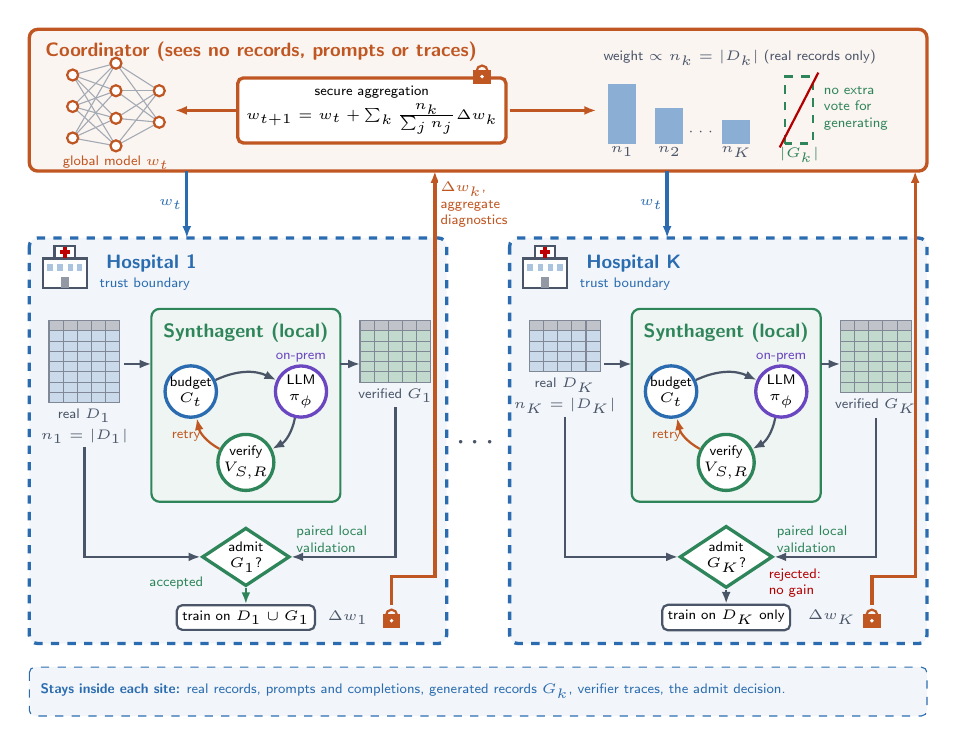
\begin{tikzpicture}[
  font=\sffamily\scriptsize,
  >={Latex[length=1.5mm]},
  flow/.style={->,thick,sgray},
  down/.style={->,very thick,sblue},
  up/.style={->,very thick,sorange},
  pan/.style={rounded corners=3pt,draw=#1,very thick,fill=#1!6},
  ttl/.style={font=\sffamily\bfseries\scriptsize,text=#1},
  lab/.style={font=\sffamily\tiny,text=#1,inner sep=1pt},
  nd/.style={circle,draw=#1,very thick,fill=white,minimum size=6.5mm,inner sep=0pt,font=\sffamily\tiny,align=center},
  diam/.style={diamond,aspect=1.5,draw=sgreen,very thick,fill=white,inner sep=0.5pt,font=\sffamily\tiny,align=center},
]
%---------------------------------------------------------------- icons
\def\lock#1#2{% padlock at (#1), colour #2
  \begin{scope}[shift={(#1)}]
    \draw[#2,thick] (-0.07,0.05) arc[start angle=180,end angle=0,radius=0.07];
    \fill[#2] (-0.11,-0.11) rectangle (0.11,0.06);
    \fill[white] (0,-0.02) circle (0.025);
  \end{scope}}
\def\hospital#1{% small hospital building at (#1)
  \begin{scope}[shift={(#1)}]
    \fill[white,draw=sgray,thick] (-0.28,-0.22) rectangle (0.28,0.16);
    \fill[white,draw=sgray,thick] (-0.13,0.16) rectangle (0.13,0.32);
    \fill[red!75!black] (-0.025,0.17) rectangle (0.025,0.31);
    \fill[red!75!black] (-0.065,0.215) rectangle (0.065,0.265);
    \foreach \x in {-0.19,-0.06,0.07,0.19}{\fill[sblue!40] (\x-0.035,0.0) rectangle ++(0.07,0.09);}
    \fill[sgray!60] (-0.05,-0.22) rectangle (0.05,-0.08);
  \end{scope}}
\def\tabl#1#2#3#4{% table glyph at (#1): #2 rows, row fill #3, highlighted row #4
  \begin{scope}[shift={(#1)}]
    \fill[sgray!35] (0,0) rectangle (0.9,-0.13);
    \foreach \r in {1,...,#2}{
      \ifnum\r=#4 \fill[sorange!45] (0,-0.13*\r) rectangle (0.9,-0.13*\r-0.13);
      \else \fill[#3] (0,-0.13*\r) rectangle (0.9,-0.13*\r-0.13);\fi}
    \foreach \c in {0,0.18,...,0.73}{\draw[sgray!70] (\c,0) rectangle ++(0.18,-0.13*#2-0.13);}
    \foreach \r in {0,...,#2}{\draw[sgray!70] (0,-0.13*\r) -- (0.9,-0.13*\r);}
  \end{scope}}
%---------------------------------------------------------------- one hospital site
% #1 x-offset, #2 site index label, #3 real rows (n_k), #4 generated rows,
% #5 admit decision text, #6 admit colour
\def\site#1#2#3#4#5#6{%
\begin{scope}[shift={(#1,0)}]
  % trust boundary
  \draw[pan=sblue,dashed] (0,0) rectangle (5.3,-5.15);
  \hospital{0.45,-0.42}
  \node[ttl=sblue,anchor=west] at (0.85,-0.32) {Hospital #2};
  \node[lab=sblue,anchor=west] at (0.85,-0.58) {trust boundary};
  % private data
  \tabl{0.25,-1.05}{#3}{sblue!25}{0}
  \node[lab=sgray,anchor=north] at (0.7,-1.05-0.13*#3-0.17) {real $D_#2$};
  \node[lab=sgray,anchor=north] at (0.7,-1.05-0.13*#3-0.42) {$n_#2=|D_#2|$};
  % local Synthagent loop
  \fill[sgreen!8,draw=sgreen,rounded corners=3pt,thick] (1.55,-0.9) rectangle (3.95,-3.35);
  \node[ttl=sgreen,anchor=north] at (2.75,-0.95) {\system{} (local)};
  \node[nd=sblue]  (b#2) at (2.05,-1.95) {budget\\$C_t$};
  \node[nd=spurple](l#2) at (3.45,-1.95) {LLM\\$\pi_\phi$};
  \node[nd=sgreen] (v#2) at (2.75,-2.85) {verify\\$V_{S,R}$};
  \draw[flow,bend left=25] (b#2) to (l#2);
  \draw[flow,bend left=25] (l#2) to (v#2);
  \draw[->,thick,sorange,bend left=25] (v#2) to node[lab=sorange,left,pos=.5]{retry} (b#2);
  \node[lab=spurple,anchor=south] at (3.45,-1.62) {on-prem};
  \draw[flow] (1.2,-1.6) -- (1.55,-1.6);
  % generated rows
  \tabl{4.2,-1.05}{#4}{sgreen!30}{0}
  \node[lab=sgray,anchor=north] at (4.65,-1.05-0.13*#4-0.17) {verified $G_#2$};
  \draw[flow] (3.95,-1.6) -- (4.2,-1.6);
  % admission gate
  \node[diam] (g#2) at (2.75,-4.05) {admit\\$G_#2$?};
  \draw[flow] (4.65,-1.05-0.13*#4-0.45) |- (g#2.east);
  \draw[flow] (0.7,-1.05-0.13*#3-0.7) |- (g#2.west);
  \node[lab=sgreen,anchor=north west,align=left] at (3.35,-3.62) {paired local\\validation};
  % local training and protected update
  \node[draw=sgray,thick,fill=white,rounded corners=2pt,font=\sffamily\tiny,align=center,inner sep=2pt]
       (t#2) at (2.75,-4.82) {train on #5};
  \draw[flow,#6] (g#2.south) -- (t#2.north);
  \node[lab=sgray,anchor=west] at (3.75,-4.82) {$\Delta w_#2$};
  \lock{4.6,-4.84}{sorange}
\end{scope}}
%================================================================ coordinator
\draw[pan=sorange] (0,2.65) rectangle (11.4,0.85);
\node[ttl=sorange,anchor=north west] at (0.08,2.62) {Coordinator (sees no records, prompts or traces)};
% global model glyph
\begin{scope}[shift={(0.55,1.12),yscale=0.85}]
  \foreach \i/\y in {1/0.15,2/0.55,3/0.95}{\coordinate (a\i) at (0,\y);}
  \foreach \i/\y in {1/0.05,2/0.4,3/0.75,4/1.1}{\coordinate (h\i) at (0.55,\y);}
  \foreach \i/\y in {1/0.35,2/0.75}{\coordinate (o\i) at (1.1,\y);}
  \foreach \a in {1,2,3}{\foreach \h in {1,2,3,4}{\draw[sgray!50] (a\a)--(h\h);}}
  \foreach \h in {1,2,3,4}{\foreach \o in {1,2}{\draw[sgray!50] (h\h)--(o\o);}}
  \foreach \p in {a1,a2,a3,h1,h2,h3,h4,o1,o2}{\fill[white,draw=sorange,thick] (\p) circle (0.07);}
  \node[lab=sorange,anchor=north] at (0.55,-0.04) {global model $w_t$};
\end{scope}
% secure aggregation
\node[draw=sorange,very thick,fill=white,rounded corners=2pt,align=center,inner sep=3pt,font=\sffamily\tiny]
  (agg) at (4.35,1.62) {secure aggregation\\[1pt]
  $w_{t+1}=w_t+\sum_k \frac{n_k}{\sum_j n_j}\Delta w_k$};
\lock{5.75,2.07}{sorange}
\draw[flow,sorange] (agg.west) -- (1.85,1.62);
% weights bars
\begin{scope}[shift={(7.35,1.2)}]
  \node[lab=sgray,anchor=south west] at (-0.1,0.95) {weight $\propto n_k=|D_k|$ (real records only)};
  \fill[sblue!55] (0,0) rectangle (0.35,0.75);   \node[lab=sgray,anchor=north] at (0.18,0) {$n_1$};
  \fill[sblue!55] (0.6,0) rectangle (0.95,0.45); \node[lab=sgray,anchor=north] at (0.78,0) {$n_2$};
  \fill[sblue!55] (1.45,0) rectangle (1.8,0.3);  \node[lab=sgray,anchor=north] at (1.63,0) {$n_K$};
  \node[lab=sgray] at (1.2,0.15) {$\cdots$};
  % ghost bar: generated rows do not count
  \draw[sgreen,dashed,thick] (2.25,0) rectangle (2.6,0.85);
  \draw[red!70!black,thick] (2.18,-0.05) -- (2.67,0.9);
  \node[lab=sgreen,anchor=north,align=center] at (2.43,0) {$|G_k|$};
  \node[lab=sgreen,anchor=west,align=left] at (2.7,0.45) {no extra\\vote for\\generating};
\end{scope}
\draw[flow,sorange] (6.1,1.62) -- (7.2,1.62);
%================================================================ sites
\site{0}{1}{7}{5}{$D_1\cup G_1$}{sgreen}
\node[font=\sffamily\bfseries\large,text=sgray] at (5.7,-2.6) {$\cdots$};
\site{6.1}{K}{4}{6}{$D_K$ only}{sgray}
\node[lab=red!70!black,anchor=west,align=left] at (6.1+3.25,-4.38) {rejected:\\no gain};
\node[lab=sgreen,anchor=east,align=right] at (2.25,-4.38) {accepted};
%================================================================ boundary crossings
\draw[down] (2.0,0.85) -- node[lab=sblue,left,align=right]{$w_t$} (2.0,0.0);
\draw[up]   (4.6,-4.66) -- (4.6,-4.3) -- (5.15,-4.3) -- (5.15,0.0) -- (5.15,0.85);
\draw[down] (8.1,0.85) -- node[lab=sblue,left,align=right]{$w_t$} (8.1,0.0);
\draw[up]   (6.1+4.6,-4.66) -- (6.1+4.6,-4.3) -- (6.1+5.15,-4.3) -- (6.1+5.15,0.85);
\node[lab=sorange,anchor=west,align=left,fill=white] at (5.18,0.42) {$\Delta w_k$,\\aggregate\\diagnostics};
%================================================================ legend
\begin{scope}[shift={(0,-5.45)}]
  \fill[sblue!6,draw=sblue,dashed,rounded corners=2pt] (0,0) rectangle (11.4,-0.62);
  \node[lab=sblue,anchor=west,align=left] at (0.1,-0.31)
    {\textbf{Stays inside each site:} real records, prompts and completions, generated records $G_k$, verifier traces, the admit decision.};
\end{scope}
\end{tikzpicture}
}
\DIFaddendFL \caption{Deployment across healthcare facilities. Each facility runs \system (context selection, a locally served LLM, validation and correction) inside its own infrastructure, then decides with paired local validation whether to use the synthetic records $G_k$ (Facility~1) or to train on real data only (Facility~$K$). Only the model update $\Delta w_k$ and approved aggregate diagnostics leave the facility. The coordinator weights each update by the number of real records $n_k=|D_k|$ (Equation~\eqref{eq:federated-aggregate}), so generating more records gives a facility no extra weight.}
\label{fig:federated}
\DIFdelbeginFL %DIFDELCMD < \end{minipage}
%DIFDELCMD < \end{figure*}
%DIFDELCMD < %%%
\DIFdelend \DIFaddbegin \end{figure}
\DIFaddend 


%======================================================================
\section{Experimental Setup}
\label{sec:setup}
%======================================================================
This section describes the data, protocol, configurations and measures used to answer RQ1 to RQ4.

\subsection{Datasets}
We use ten public classification datasets (Table~\ref{tab:datasets}): six widely used benchmarks, five from the UCI repository~\cite{uciheart,ucibreast,uciheartfailure,uciilpd,uciparkinsons} and the Pima Indians diabetes data~\cite{smith1988diabetes}, and four further UCI datasets that are smaller, have missing values or mixed types, or are imbalanced~\cite{patricio2018coimbra,ucihepatitis,ucickd,zieba2014thoracic}. Each has fewer training records than the minimum sample size recommended for developing a prediction model for its task by the criteria of Riley et al.~\cite{riley2019binary}. Together they span the factors that make small data a challenge for the classifier: 116 to 768 records, 8 to 30 features, two to five classes, a smallest class from 4.3\% to 44.8\% of the records and up to 10.1\% missing values. We keep the original five-class heart-disease target, code the targets of the four further datasets as 0/1 and their binary categories as 0/1, and impute missing values with the mean for numerical and the mode for categorical features, separately within each \DIFdelbegin \DIFdel{training and test split}\DIFdelend \DIFaddbegin \DIFadd{division}\DIFaddend . The control-layer variants, the \DIFaddbegin \DIFadd{other }\DIFaddend LLM variants and the sensitivity study use the six original datasets; the main configurations and all established generators use all ten.

\begin{table}[t]
\centering
\caption{Evaluation datasets. $n$: records; $d$: features; $k$: classes; $n_{\min}$: records in the smallest class; $n^{\star}$: minimum sample size by the first criterion of Riley et al.~\cite{riley2019binary} (shrinkage 0.9, $d(k-1)$ parameters, anticipated $R^2_{\mathrm{CS}}$ of 15\% of its maximum); Ratio: $n^{\star}/n_{\mathrm{tr}}$, with $n_{\mathrm{tr}}=0.8n$ the training size.}
\label{tab:datasets}
\footnotesize
\setlength{\tabcolsep}{3pt}
\begin{tabular*}{\columnwidth}{@{\extracolsep{\fill}}lrrrrrr@{}}
\toprule
Dataset & $n$ & $d$ & $k$ & $n_{\min}$ (\%) & $n^{\star}$ & Ratio \\
\midrule
Heart disease & 303 & 13 & 5 & 13 (4.3) & 10,201 & 42.1 \\
Breast cancer & 569 & 30 & 2 & 212 (37.3) & 2,302 & 5.1 \\
Heart failure & 299 & 12 & 2 & 96 (32.1) & 946 & 4.0 \\
Diabetes & 768 & 8 & 2 & 268 (34.9) & 621 & 1.0 \\
Liver disease & 583 & 10 & 2 & 167 (28.6) & 808 & 1.7 \\
Parkinson's & 195 & 22 & 2 & 48 (24.6) & 1,851 & 11.9 \\
Breast cancer (C.) & 116 & 9 & 2 & 52 (44.8) & 677 & 7.3 \\
Hepatitis & 155 & 19 & 2 & 32 (20.6) & 1,688 & 13.6 \\
Kidney disease & 400 & 24 & 2 & 150 (37.5) & 1,840 & 5.8 \\
Thoracic surgery & 470 & 16 & 2 & 70 (14.9) & 1,606 & 4.3 \\
\bottomrule
\end{tabular*}
\par\vspace{2pt}\raggedright\scriptsize For heart disease, $n^{\star}$ applies the binary criterion to the smallest class versus the rest and is an approximation. Parkinson's contains several recordings per subject, so its effective number of independent records is lower and its ratio higher than shown.
\end{table}

\subsection{Protocol}
Measuring whether synthetic records help a classifier requires real records that the generator has never seen. Each dataset is therefore divided into a training set, given to the generator, and a test set of 20\% of the records, used only to score classifiers. Because a test set of 24 to 154 records makes a single division unreliable, the division is repeated ten times with different random seeds, and means and standard deviations are reported. In each repetition, the number of synthetic records $N$ equals the number of training records, so augmentation doubles the training set; because records are requested in batches of at most $b=30$, a generator that falls short does so on small requests, not because $N$ is large. Ten classifiers covering the main model families are trained: logistic regression (LR), support vector machine (SVM), $k$-nearest neighbours ($k$NN), Gaussian naive Bayes (NB), decision tree (DT), random forest (RF), gradient boosting (GB), AdaBoost, XGBoost and a multilayer perceptron (MLP), with library defaults except the number of neighbours, tree depth and number of estimators, which scale with the training size. Using several families avoids conclusions tied to one learner, since interpolated records can help a nearest-neighbour classifier and harm a boosted ensemble. Each classifier is trained in three setups, (1) on real records only, (2) on synthetic records only and (3) on real plus synthetic records, and all three are scored on the same test set. XGBoost failed on liver disease in every repetition because it requires classes coded from 0, whereas this dataset codes them as $\{1,2\}$, so 99 of the 100 classifier-dataset combinations are reported.

\subsection{Configurations}
Table~\ref{tab:configs} lists the 36 configurations. A configuration is included in the analysis only if it completed all its datasets and ten repetitions. The \emph{reference} configuration is \system with its default settings and GPT-4o mini, the least expensive LLM; every other configuration differs from it in one respect. The \emph{direct-prompting} baseline uses the same LLM, prompts and context, but none of the control layer: no repair, correction, retry or completion loop. The \emph{structured-output} baseline adds to it the provider's strict JSON-schema mode, which constrains decoding to the column names, numerical types and observed categories of the real data but does not bound the number of records. The \emph{CLLM} baseline follows direct prompting with the curation step of CLLM~\cite{seedat2024cllm}, which keeps only the records that an XGBoost model trained on the real data learns with confidence of at least 0.75 and aleatoric uncertainty of at most 0.2 (the Data-IQ criteria~\cite{seedat2022dataiq}). Eight control-layer variants change one component or repeat the reference run, and three LLM variants replace GPT-4o mini, forming a $2\times2$ design that crosses model generation (4o versus 4.1) with model size (mini versus full). A second provider, Anthropic, adds three LLMs under the reference configuration, Claude Haiku 4.5, Claude Sonnet 4.6 and Claude Sonnet 5.5, and repeats both baselines with Claude Haiku 5.5, used for the baselines only because its \system run did not complete (Section~\ref{sec:rq1}). The Claude models run without extended reasoning and at their default temperature, which the newest of them do not allow to be changed, whereas the OpenAI models use the temperature of Table~\ref{tab:params}. Token counts are compared only within a provider, because the tokenizers differ. Six sensitivity variants change one parameter of Table~\ref{tab:params} at a time. Ten established generators cover the other families, all with the default settings of their reference implementations and the same divisions; the oversampling methods balance the classes, so their number of records follows the class balance, whereas the others sample $N$ records: oversampling (SMOTE~\cite{chawla2002smote}, ADASYN~\cite{he2008adasyn}, Borderline-SMOTE~\cite{han2005borderline}), statistical (a Gaussian copula~\cite{patki2016sdv} and a discrete Bayesian network learned by hill climbing~\cite{zhang2014privbayes}), tree-based (sequential CART synthesis~\cite{nowok2016synthpop} and adversarial random forests, ARF~\cite{watson2023arf}) and deep (CTGAN, TVAE~\cite{xu2019ctgan} and TabDDPM~\cite{kotelnikov2023tabddpm}). In total, the configurations give 2,800 dataset-configuration repetitions and up to 84,000 classifier fits.

\begin{table}[t]
\centering
\caption{The 36 evaluated configurations. \DIFdelbeginFL \DIFdelFL{All }\DIFdelendFL LLM configurations use GPT-4o mini \DIFdelbeginFL \DIFdelFL{, except the }\DIFdelendFL \DIFaddbeginFL \DIFaddFL{unless another }\DIFaddendFL LLM \DIFdelbeginFL \DIFdelFL{variants and the baselines repeated with Claude Haiku 5.5}\DIFdelendFL \DIFaddbeginFL \DIFaddFL{is named}\DIFaddendFL . $^{\ast}$Run on all ten datasets; the others on the six original ones.}
\label{tab:configs}
\footnotesize
\DIFdelbeginFL %DIFDELCMD < \setlength{\tabcolsep}{2pt}
%DIFDELCMD < \begin{tabular}{@{}p{.23\columnwidth}p{.31\columnwidth}r@{\hspace{4pt}}p{.33\columnwidth}@{}}
%DIFDELCMD < \toprule
%DIFDELCMD < Group & Configurations & No. & Purpose \\
%DIFDELCMD < \midrule
%DIFDELCMD < Baselines (RQ1) & Direct prompting and structured outputs, with GPT-4o mini$^{\ast}$ and Claude Haiku 5.5; CLLM$^{\ast}$ & 5 & Same LLM without the control layer: free or schema-constrained decoding, or a curation filter \\
%DIFDELCMD < Reference & \system, default settings$^{\ast}$ & 1 & Point of comparison for all others \\
%DIFDELCMD < Repeated runs (RQ1) & No type rules; no post-processing; no context join; logged rerun & 4 & Change nothing in this setting; estimate the variation between runs \\
%DIFDELCMD < Design choices (RQ1) & Dense context; diverse context; LLM-chosen settings; range enforcement & 4 & Effect of context selection, of letting the LLM set $\rho$ and the temperature, and of clipping values to the observed ranges \\
%DIFDELCMD < Sensitivity (RQ1) & $\rho$ of 10\% and 40\%; $b$ of 15 and 60; temperature 0 and 1.0 & 6 & Effect of each fixed parameter \\
%DIFDELCMD < LLM variants (RQ4) & GPT-4.1 mini; GPT-4o; GPT-4.1$^{\ast}$; Claude Haiku 4.5; Claude Sonnet 4.6$^{\ast}$; Claude Sonnet 5.5 & 6 & Effect of model generation, size and provider \\
%DIFDELCMD < Established generators$^{\ast}$ (RQ4) & SMOTE; ADASYN; Borderline-SMOTE; Gaussian copula; Bayesian network; CART; ARF; CTGAN; TVAE; TabDDPM & 10 & Generators fitted to the real records \\
%DIFDELCMD < \midrule
%DIFDELCMD < Total & & 36 & \\
%DIFDELCMD < \bottomrule
%DIFDELCMD < \end{tabular}
%DIFDELCMD < %%%
\DIFdelendFL \DIFaddbeginFL \setlength{\tabcolsep}{3pt}
\renewcommand{\arraystretch}{1.15}
\begin{tabular}{@{}>{\raggedright\arraybackslash}p{.30\columnwidth}>{\raggedright\arraybackslash}p{.60\columnwidth}r@{}}
\toprule
Group & Configurations & No. \\
\midrule
\multicolumn{3}{@{}l}{\textit{Control layer (RQ1)}}\\
Reference & \system, default settings$^{\ast}$ & 1 \\
Baselines: no control layer & Direct prompting and structured outputs (GPT-4o mini$^{\ast}$, Claude Haiku 5.5); CLLM$^{\ast}$ & 5 \\
Repeated runs: noise floor & No type rules; no post-processing; no context join; logged rerun & 4 \\
Design choices & Dense or diverse context; LLM-chosen settings; range enforcement & 4 \\
Sensitivity & $\rho$: 10\%, 40\%; $b$: 15, 60; temperature: 0, 1 & 6 \\
\midrule
\multicolumn{3}{@{}l}{\textit{Comparison (RQ4)}}\\
LLM variants & GPT-4.1 mini, GPT-4o, GPT-4.1$^{\ast}$; Claude Haiku 4.5, Sonnet 4.6$^{\ast}$, Sonnet 5.5 & 6 \\
Established generators$^{\ast}$ & Oversampling: SMOTE, ADASYN, Borderline-SMOTE. Statistical: Gaussian copula, Bayesian network. Tree-based: CART, ARF. Deep: CTGAN, TVAE, TabDDPM & 10 \\
\midrule
Total & & 36 \\
\bottomrule
\end{tabular}
\DIFaddendFL \end{table}

Three of the control-layer variants change nothing in this setting: with no user rules, disabling post-processing removes a step that does nothing, the context join does not change the records, and disabling type rules cannot change the output because the validator never found a type violation with GPT-4o mini. Together with the reference and a rerun of it that only adds per-request logging, they are five independent runs of the same pipeline, and their spread estimates the variation between repeated runs, which we call the \emph{noise floor}: a difference between two configurations that is smaller than this spread is not evidence of an effect.

\subsection{Measures}
Each research question has its own measures, all computed on every repetition: integrity for RQ1, fidelity and privacy for RQ2, and utility for RQ3 and RQ4, with cost reported throughout. \emph{Integrity} is measured by the records delivered against those requested, the non-empty values, the malformed responses and the corrections. \emph{Fidelity} compares the synthetic records alone with the real training records over the numerical features $\mathcal{J}$:
\begin{equation}
\begin{aligned}
F_{\mathrm{JSD}}&=100\Bigl(1-\tfrac{1}{|\mathcal{J}|}
\textstyle\sum_{j\in\mathcal{J}}D_{\mathrm{JS}}(D_j,G_j)\Bigr),\\
F_{\mathrm{corr}}&=100\bigl(1-\operatorname{mean}|\Sigma_D-\Sigma_G|\bigr),
\end{aligned}
\label{eq:fidelity}
\end{equation}
where \DIFaddbegin \DIFadd{$D_j$ and $G_j$ are the values of feature $j$ in the real and synthetic records, }\DIFaddend $D_{\mathrm{JS}}$ is the Jensen-Shannon divergence between \DIFdelbegin \DIFdel{real and synthetic distributionsof a feature }\DIFdelend \DIFaddbegin \DIFadd{their distributions, }\DIFaddend and $\Sigma_D$, $\Sigma_G$ are the correlation matrices; both scores equal 100 for identical distributions. A classifier two-sample test (C2ST)~\cite{lopezpaz2017c2st} trains a random forest to separate real from synthetic records; an accuracy close to 0.5 means they are hard to tell apart. \emph{Privacy} is measured by a membership-inference attack that scores each real record by its distance to the nearest synthetic record and reports the ROC AUC between training and test records, where 0.5 is chance, and by the share of \emph{near-copies}, synthetic records within Euclidean distance 0.05 of a real record over the min-max-scaled numerical features (first 200 synthetic records of each run). \emph{Utility} is the paired change, for metric $m\in\{\mathrm{accuracy},\mathrm{F1}\}$, dataset $d$, classifier $c$ and repetition $h$,
\begin{equation}
\Delta m_{d,c,h}=m\bigl(D_{d,h}\cup G_{d,h};\,c\bigr)-m\bigl(D_{d,h};\,c\bigr),
\label{eq:utility}
\end{equation}
\DIFaddbegin \DIFadd{where $D_{d,h}$ and $G_{d,h}$ are the real training records and the synthetic records of dataset $d$ in repetition $h$, and $m(\cdot;c)$ is the score of classifier $c$ trained on them, }\DIFaddend with both models scored on the same test set. We use binary F1 for the binary tasks and class-weighted F1 for heart disease, and report changes in percentage points (pp).

\subsection{Statistical Analysis}
Repetitions and classifiers are not independent datasets, so they are averaged within each dataset and the datasets are treated as matched blocks. Configurations are compared with the Friedman test,
\begin{equation}
\chi^2_F=\frac{12M}{Q(Q+1)}\sum_{a=1}^{Q}\bar{\mathrm{rk}}_a^{\,2}-3M(Q+1),
\label{eq:friedman}
\end{equation}
where $\bar{\mathrm{rk}}_a$ is the average rank of configuration $a$ over $M$ datasets (six or ten) and $Q$ the number of configurations, followed by two-sided Wilcoxon signed-rank tests of the best-ranked configuration against every other, with Holm correction~\cite{demsar2006statistical,holm1979procedure}. With few blocks the tests have limited power, so effect sizes and the noise floor are reported alongside $p$-values. As a sensitivity analysis, the comparison of LLMs is repeated with the 60 matched dataset-division pairs as blocks; these share records, so the dataset-level tests remain the primary analysis.

%======================================================================
\section{Results}
\label{sec:results}
\begin{table}[t]
\centering
\caption{Results at a glance over the ten datasets: ranges over the three LLMs of \system, the three other LLM-based generators and the ten established generators. Only \system has no integrity violations, and it reaches the largest median F1 gain. \DIFaddbeginFL \DIFaddFL{Bold: where }\system \DIFaddFL{is best.}\DIFaddendFL }
\label{tab:glance}
\scriptsize
\setlength{\tabcolsep}{1.5pt}
\DIFdelbeginFL %DIFDELCMD < \begin{tabular*}{\columnwidth}{@{\extracolsep{\fill}}lccc@{}}
%DIFDELCMD < \toprule
%DIFDELCMD < & \system & Other LLM & Established \\
%DIFDELCMD < \midrule
%DIFDELCMD < Integrity violations & none & 13-22\% missing & no LLM \\
%DIFDELCMD < Malformed responses & repaired & batches lost & - \\
%DIFDELCMD < Near-copies (\%) & 6-9 & 4-7 & 1-19 \\
%DIFDELCMD < Attack AUC & 0.51-0.52 & 0.51-0.52 & 0.50-0.57 \\
%DIFDELCMD < Fidelity (JSD) & 72-77 & 66-72 & 62-86 \\
%DIFDELCMD < Median $\Delta$F1 (pp) & $-0.69$ to \best{$+1.43$} & $-0.68$ to $+0.24$ & $-2.15$ to $+0.11$ \\
%DIFDELCMD < Tokens per record & $-17\%$ vs.\ direct & - & no LLM \\
%DIFDELCMD < \bottomrule
%DIFDELCMD < \end{tabular*}
%DIFDELCMD < %%%
\DIFdelendFL \DIFaddbeginFL \begin{tabular*}{\columnwidth}{@{\extracolsep{\fill}}lccc@{}}
\toprule
& \system & Other LLM & Established \\
\midrule
Integrity violations & \best{none} & 13-22\% missing & no LLM \\
Malformed responses & \best{repaired} & batches lost & - \\
Near-copies (\%) & 6-9 & 4-7 & 1-19 \\
Attack AUC & 0.51-0.52 & 0.51-0.52 & 0.50-0.57 \\
Fidelity (JSD) & 72-77 & 66-72 & 62-86 \\
Median $\Delta$F1 (pp) & $-0.69$ to \best{$+1.43$} & $-0.68$ to $+0.24$ & $-2.15$ to $+0.11$ \\
Tokens per record & \best{$-17\%$} vs.\ direct & - & no LLM \\
\bottomrule
\end{tabular*}
\DIFaddendFL \end{table}
\DIFaddbegin \DIFadd{This section answers the four research questions in turn, and }\DIFaddend Table~\ref{tab:glance} summarizes the results\DIFdelbegin \DIFdel{; the subsections detail them by research question}\DIFdelend \DIFaddbegin \DIFadd{. Section~\ref{sec:rq1} shows that the control layer delivers the requested dataset where the LLM alone does not (Figure~\ref{fig:delivery}) and that its settings change cost and fidelity but not utility (Figure~\ref{fig:ablation}). Section~\ref{sec:rq2} measures how closely the records follow the real data and whether they expose real patients, Section~\ref{sec:rq3} their effect on each classifier (Figure~\ref{fig:heatmap}), and Section~\ref{sec:rq4} compares }\system \DIFadd{with the other generators and LLMs (Figure~\ref{fig:radar})}\DIFaddend .
%======================================================================
\subsection{RQ1: Control Layer and Integrity}
\label{sec:rq1}
\textbf{Finding~1.} The control layer ensures integrity: without it, every run of the same LLM missed or added records; with it, no logged run had an integrity violation\DIFdelbegin \DIFdel{, at 1.9\% more tokens in total and with unchanged fidelity}\DIFdelend . Figure~\ref{fig:delivery} shows the \DIFdelbegin \DIFdel{records delivered per dataset. On the six original datasets, direct prompting delivered 87.6}\DIFdelend \DIFaddbegin \DIFadd{gap. Direct prompting delivered 87}\DIFaddend \% of the \DIFdelbegin \DIFdel{configured records , fell short in 50 of 60 runs and overshot in the other 10, and lost an entire }\DIFdelend \DIFaddbegin \DIFadd{requested records on average and lost a whole }\DIFaddend batch to each \DIFdelbegin \DIFdel{of ten malformed responses. Fidelity, privacy and utility were the same for both configurations (JSD 72.7; attack AUC 0.517 versus 0.526; F1 change $-0.04$ versus $-0.14$ pp, within the noise floor below), so the difference lies in the integrity of the dataset. }%DIFDELCMD < 

%DIFDELCMD < %%%
\DIFdelend \DIFaddbegin \DIFadd{malformed response. }\DIFaddend Structured outputs, \DIFdelbegin \DIFdel{the providers' option to }\DIFdelend \DIFaddbegin \DIFadd{which }\DIFaddend force every response into a fixed format, \DIFdelbegin \DIFdel{do not replace the control layer (Figure~\ref{fig:delivery}). Every response had the declared columns and types, but the LLM returned on average 77.7\% of the configured records }\DIFdelend \DIFaddbegin \DIFadd{delivered 78\% }\DIFaddend and never the full dataset, \DIFdelbegin \DIFdel{at 21\% more tokens in total than }%DIFDELCMD < \system%%%
\DIFdel{. Forcing the format also }\DIFdelend \DIFaddbegin \DIFadd{and }\DIFaddend weakened the relationships between features\DIFdelbegin \DIFdel{(correlation fidelity 63.0 versus 72.6) and made the records easier to tell from real ones (C2ST 0.943 versus 0.878), while utility did not differ (Friedman $p=.311$ for F1). A fixed format therefore }\DIFdelend \DIFaddbegin \DIFadd{: a fixed format }\DIFaddend guarantees the shape of each record, but not \DIFdelbegin \DIFdel{the numberof records, which is what the completion loop provides. The same holds for the second provider: with Claude Haiku 5.5, direct prompting delivered 67.1\% of the configured records, with 294 malformed responses, and structured outputs 82.9\%. Under the control layer, the same model refused to imitate patient records in 39 of 60 repetitions; }%DIFDELCMD < \system %%%
\DIFdel{logged each refusal, but the run finished only heart failure and is excluded}\DIFdelend \DIFaddbegin \DIFadd{their number}\DIFaddend .

\begin{figure}[t]
\centering
\assetfigure{\columnwidth}{generated/delivery.pdf}
\caption{Only \system has no integrity violations (RQ1); the LLM baselines miss or add records on every dataset. Records delivered as a percentage of those requested, averaged over ten divisions\DIFaddbeginFL \DIFaddFL{; values above 100\% are responses with more records than requested}\DIFaddendFL . Baselines use GPT-4o mini; \system points are every run with a logged count (GPT-4o mini and GPT-4.1 on the four further datasets, Claude Sonnet 4.6 on all ten).}
\label{fig:delivery}
\end{figure}

\DIFdelbegin \DIFdel{These comparisons isolate the control layer's contribution, because the }\DIFdelend \DIFaddbegin \DIFadd{With the same }\DIFaddend LLM, prompts and context\DIFdelbegin \DIFdel{are the same in each pair. Its contribution is integrity , }\DIFdelend \DIFaddbegin \DIFadd{, the difference in integrity is significant (exact McNemar test on 40 paired runs, $p<10^{-11}$) and comes }\DIFaddend at no cost\DIFdelbegin \DIFdel{in utility: with GPT-4o mini, }%DIFDELCMD < \system %%%
\DIFdel{had no integrity violation in any logged run, while direct prompting missed 13\% of the records and structured outputs 22\% over ten datasets, and turned malformed responses into records instead of losing them, while the }\DIFdelend \DIFaddbegin \DIFadd{: fidelity, privacy and utility did not change (median }\DIFaddend F1 \DIFdelbegin \DIFdel{change of the two did not differ (median }\DIFdelend difference $+0.08$ pp, \DIFdelbegin \DIFdel{Wilcoxon }\DIFdelend $p=.92$)\DIFdelbegin \DIFdel{. On the 40 paired runs with logged counts, the difference in integrity is significant (exact McNemar test, $p<10^{-11}$)}\DIFdelend , and \system needed 17\% fewer tokens per delivered record than direct prompting\DIFdelbegin \DIFdel{and 40\% fewer than structured outputs (Wilcoxon $p<10^{-6}$)}\DIFdelend , because the baselines pay for records they lose.
\DIFdelbegin \DIFdel{The results therefore come from the two together: integrity is due to }\DIFdelend \DIFaddbegin 

\DIFadd{Inside }\DIFaddend the control layer, \DIFdelbegin \DIFdel{which achieved it with every LLM whose run completed while no LLM achieved it alone, and the utility gains come from the LLM's knowledge, which the control layer turns into a usable dataset (Section~\ref{sec:rq4}).
}%DIFDELCMD < 

%DIFDELCMD < %%%
\DIFdel{The design choices inside the control layer }\DIFdelend \DIFaddbegin \DIFadd{the design choices }\DIFaddend matter much less than the \DIFdelbegin \DIFdel{control }\DIFdelend layer itself (Figure~\ref{fig:ablation}). \DIFdelbegin \DIFdel{The five repeated }\DIFdelend \DIFaddbegin \DIFadd{Five }\DIFaddend runs of the same pipeline differ by up to \DIFdelbegin \DIFdel{0.5 JSD points, 2 correlation points and }\DIFdelend 0.7 pp of utility, \DIFdelbegin \DIFdel{which is }\DIFdelend the noise floor\DIFdelbegin \DIFdel{. Dense context stays inside it; diverse context slightly improves fidelity at a slightly higher attack AUC (0.544); LLM-chosen settings cost 57\% more tokens; and range enforcement lowers JSD fidelity by 0.9 points. The Friedman tests find no difference in utility between the variants ($p=.843$ for accuracy, $p=.872$ for F1}\DIFdelend \DIFaddbegin \DIFadd{, and no variant or parameter moves utility beyond it (Friedman $p\ge.17$}\DIFaddend ). The parameters \DIFdelbegin \DIFdel{of Table~\ref{tab:params} behave the same way: changing the context sample, the batch size or the temperature leaves utility within the noise floor ($p=.986$ accuracy, $p=.178$ F1), but it changes }\DIFdelend \DIFaddbegin \DIFadd{change }\DIFaddend cost and fidelity \DIFdelbegin \DIFdel{. Halving the context sample saves 27\% of the tokens and }\DIFdelend \DIFaddbegin \DIFadd{instead: }\DIFaddend doubling the batch size \DIFaddbegin \DIFadd{saves }\DIFaddend 39\% \DIFdelbegin \DIFdel{, whereas smaller batches cost 73\% more. A }\DIFdelend \DIFaddbegin \DIFadd{of the tokens, and a }\DIFaddend temperature of 1.0 raises \DIFdelbegin \DIFdel{JSD fidelity by 3.2 points and correlation fidelity by 8.7 points(C2ST 0.799 against 0.878) at no cost in utility, privacy or tokens}\DIFdelend \DIFaddbegin \DIFadd{fidelity by 3 to 9 points}\DIFaddend , so the default of 0.3 is conservative\DIFdelbegin \DIFdel{for fidelity}\DIFdelend .

\begin{figure*}[t]
\centering
\assetfigure{\textwidth}{generated/ablation_effects.pdf}
\caption{No design choice or parameter moves utility beyond the noise floor; the parameters change only cost and fidelity (RQ1). GPT-4o mini, six original datasets. The first five rows rerun the same pipeline; grey band: noise floor (reference, blue line, $\pm$ their spread); orange: outside it.}
\label{fig:ablation}
\end{figure*}



\DIFdelbegin \DIFdel{The corrections make a less disciplined LLM usable. }\DIFdelend \DIFaddbegin \DIFadd{Two observations qualify this result. The corrections matter only for less disciplined LLMs: }\DIFaddend GPT-4o mini produced no type violation, \DIFdelbegin \DIFdel{and the local parser fixed every defect in its responses. }\DIFdelend \DIFaddbegin \DIFadd{whereas }\DIFaddend GPT-4.1 mini \DIFdelbegin \DIFdel{, the fastest LLM, produced on average }\DIFdelend \DIFaddbegin \DIFadd{produced }\DIFaddend 7.4 \DIFdelbegin \DIFdel{type violations }\DIFdelend per repetition on breast cancer\DIFdelbegin \DIFdel{and one malformed response; these were sent back for correction instead of }\DIFdelend \DIFaddbegin \DIFadd{, all corrected before }\DIFaddend entering the dataset\DIFdelbegin \DIFdel{, and its datasets had no integrity violations and gave the best accuracy change of the OpenAI LLMs (Section~\ref{sec:rq4})}\DIFdelend \DIFaddbegin \DIFadd{. And a provider's safety behaviour can block generation: with Claude Haiku 5.5 the baselines delivered 67\% and 83\% of the records, and under the control layer the model refused to imitate patient records in 39 of 60 repetitions, so that run is excluded. The results therefore come from the two together: integrity is due to the control layer, and the utility gains come from the LLM's knowledge, which the control layer turns into a usable dataset}\DIFaddend .

\subsection{RQ2: Fidelity and Privacy}
\label{sec:rq2}
\textbf{Finding~2.} The generated records follow the real distributions reasonably well \DIFdelbegin \DIFdel{without revealing the real records}\DIFdelend \DIFaddbegin \DIFadd{and do not expose the real patients}\DIFaddend , but they remain distinguishable from \DIFdelbegin \DIFdel{them (Table~\ref{tab:full}). Fidelity }\DIFdelend \DIFaddbegin \DIFadd{real records. With GPT-4o mini, fidelity }\DIFaddend averages 72.7 out of 100, from 65.2 on heart disease, the \DIFaddbegin \DIFadd{dataset }\DIFaddend furthest below its required sample size, to 80.2 on diabetes, the closest. The membership-inference attack stays near chance \DIFdelbegin \DIFdel{(AUC 0.526 on average, }\DIFdelend \DIFaddbegin \DIFadd{on every dataset (AUC }\DIFaddend at most 0.567), \DIFdelbegin \DIFdel{which is a diagnostic for one attack rather than a formal guarantee. The records are also not interpolations of training patients: }\DIFdelend \DIFaddbegin \DIFadd{and }\DIFaddend 7.8\% \DIFaddbegin \DIFadd{of the records }\DIFaddend are near-copies \DIFaddbegin \DIFadd{of real ones}\DIFaddend , against 17-19\% for \DIFdelbegin \DIFdel{the oversampling methods and comparable to the }\DIFdelend \DIFaddbegin \DIFadd{oversampling and }\DIFaddend 1-8\% \DIFdelbegin \DIFdel{of the statistical, tree-based and deep generators. Nor do the LLMs }\DIFdelend \DIFaddbegin \DIFadd{for the other fitted generators. The LLMs do not appear to }\DIFaddend recall the public datasets \DIFaddbegin \DIFadd{either}\DIFaddend : near-copies of held-out test records, never shown to the LLM, are rarer \DIFdelbegin \DIFdel{(2.6-4.1\%) than of an equal-sized training sample (3.7-5.0\%)}\DIFdelend \DIFaddbegin \DIFadd{than those of training records}\DIFaddend , as for the fitted generators. A classifier can still \DIFdelbegin \DIFdel{separate }\DIFdelend \DIFaddbegin \DIFadd{tell }\DIFaddend real from synthetic records (C2ST 0.878), so synthetic records complement real ones rather than replace them.



\DIFdelbegin %DIFDELCMD < \begin{table}[t]
%DIFDELCMD < \centering
%DIFDELCMD < %%%
%DIFDELCMD < \caption{%
{%DIFAUXCMD
\DIFdelFL{The synthetic records follow the real distributions and keep the attack near chance on every dataset (RQ2, RQ3). Reference configuration (GPT-4o mini) per original dataset, over ten repetitions and all classifiers; JSD and correlation on a 0-100 scale.}}
%DIFAUXCMD
%DIFDELCMD < \label{tab:full}
%DIFDELCMD < \footnotesize
%DIFDELCMD < \setlength{\tabcolsep}{2.2pt}
%DIFDELCMD < \begin{tabular*}{\columnwidth}{@{\extracolsep{\fill}}lrrrrrrrr@{}}
%DIFDELCMD < \toprule
%DIFDELCMD < & \multicolumn{4}{c}{Fidelity and privacy} & \multicolumn{2}{c}{Acc.\ (\%)} & \multicolumn{2}{c}{Change (pp)} \\
%DIFDELCMD < \cmidrule(lr){2-5}\cmidrule(lr){6-7}\cmidrule(l){8-9}
%DIFDELCMD < Dataset & JSD & Corr. & C2ST & AUC & Real & Aug. & Acc. & F1 \\
%DIFDELCMD < \midrule
%DIFDELCMD < Breast & 77.2 & 74.5 & 0.911 & 0.550 & 95.1 & 94.4 & $-0.66$ & $-0.62$ \\
%DIFDELCMD < Diabetes & 80.2 & 44.0 & 0.897 & 0.504 & 74.2 & 74.1 & $-0.03$ & $+2.39$ \\
%DIFDELCMD < Heart dis. & 65.2 & 76.6 & 0.893 & 0.507 & 56.6 & 53.4 & $-3.15$ & $-0.97$ \\
%DIFDELCMD < Heart fail. & 71.2 & 81.2 & 0.892 & 0.534 & 74.1 & 71.6 & $-2.53$ & $-1.00$ \\
%DIFDELCMD < Liver & 71.8 & 73.8 & 0.883 & 0.495 & 67.4 & 67.6 & $+0.19$ & $+0.13$ \\
%DIFDELCMD < Parkinson's & 70.6 & 85.3 & 0.789 & 0.567 & 84.9 & 84.0 & $-0.97$ & $-0.77$ \\
%DIFDELCMD < \midrule
%DIFDELCMD < Mean & 72.7 & 72.6 & 0.878 & 0.526 & 75.4 & 74.2 & $-1.19$ & $-0.14$ \\
%DIFDELCMD < \bottomrule
%DIFDELCMD < \end{tabular*}
%DIFDELCMD < \end{table}
%DIFDELCMD < 

%DIFDELCMD < %%%
\DIFdelend \subsection{RQ3: Utility for Classifiers Trained on Small Data}
\label{sec:rq3}
\textbf{Finding~3.} The generated records help the classifiers that fail on the minority class and slightly harm those that are already strong \DIFdelbegin \DIFdel{, so their effect depends on the dataset and the classifier}\DIFdelend \DIFaddbegin \DIFadd{(Figure~\ref{fig:heatmap})}\DIFaddend . On heart failure, for example, \DIFdelbegin \DIFdel{SVM and }\DIFdelend $k$NN \DIFdelbegin \DIFdel{reach over 60\% accuracy with an F1 of almost zero because they rarely predict }\DIFdelend \DIFaddbegin \DIFadd{predicts }\DIFaddend the minority class \DIFdelbegin \DIFdel{. With the reference configuration}\DIFdelend \DIFaddbegin \DIFadd{so rarely that its F1 is almost zero, and synthetic records raise it by 15.3 pp. With GPT-4o mini}\DIFaddend , F1 improves in 26 of the 59 classifier-dataset combinations and decreases in 31\DIFdelbegin \DIFdel{(Figure~\ref{fig:heatmap}); the largest gains occur where real-only training fails, such as $k$NN on heart failure ($+15.3$ F1 points). No combination is significant }\DIFdelend \DIFaddbegin \DIFadd{, none significantly }\DIFaddend after Holm correction\DIFaddbegin \DIFadd{, so the average effect is nil ($-0.14$ pp)}\DIFaddend . Trained on synthetic records alone, classifiers keep a median 85-98\% of their real-only F1, close to the statistical and tree-based generators\DIFdelbegin \DIFdel{(92-99\%). On average, F1 is unchanged with GPT-4o mini ($-0.14$ pp) andgains more with stronger LLMs (Section~\ref{sec:rq4})}\DIFdelend \DIFaddbegin \DIFadd{. The effect therefore depends on the classifier and, as the next section shows, on the LLM}\DIFaddend .



\begin{figure*}[t]
\centering
\assetfigure{\textwidth}{generated/utility_heatmap.pdf}
\caption{The synthetic records help the classifiers that fail on real data alone and slightly harm strong ones (RQ3). Change from real-only to real-plus-synthetic training, reference configuration, per classifier and dataset; hatched: not evaluated.}
\label{fig:heatmap}
\end{figure*}



\begin{figure*}[t]
\centering
\assetfigure{\textwidth}{generated/radar_f1.pdf}
\caption{\system gains most where real-only training is weak; oversampling swings most (RQ4). F1 change (pp) per dataset for every generator, one panel per group, each against \system \DIFdelbeginFL \DIFdelFL{with Claude Sonnet 4.6 }\DIFdelendFL (dark blue)\DIFdelbeginFL \DIFdelFL{; }\DIFdelendFL \DIFaddbeginFL \DIFaddFL{. Rings from the centre: $-10$, $0$ (dashed) and $+10$ pp, on a }\DIFaddendFL symmetric logarithmic \DIFdelbeginFL \DIFdelFL{radius }\DIFdelendFL \DIFaddbeginFL \DIFaddFL{scale }\DIFaddendFL (linear within $\pm1$ pp)\DIFdelbeginFL \DIFdelFL{; dashed circle: no change}\DIFdelendFL \DIFaddbeginFL \DIFaddFL{. The LLM-based baselines use GPT-4o mini}\DIFaddendFL .}
\label{fig:radar}
\end{figure*}

\DIFaddbegin \begin{figure}[t]
\centering
\assetfigure{\columnwidth}{generated/tradeoff.pdf}
\caption{\system \DIFaddFL{gives the largest utility gain, and the statistical and tree-based generators the highest fidelity (RQ4). Median F1 change against fidelity over the ten datasets, one point per generator; dashed line: no change. The LLM-based baselines use GPT-4o mini.}}
\label{fig:tradeoff}
\end{figure}

\DIFaddend \subsection{RQ4: Comparison with Established Generators and LLMs}
\label{sec:rq4}
\begin{table}[t]
\centering
\caption{Under the control layer, no LLM produced an integrity violation in any logged run; the Claude models give the highest fidelity and F1 gain (RQ4). Reference configuration; seconds and tokens are means per repetition\DIFdelbeginFL \DIFdelFL{, }\DIFdelendFL \DIFaddbeginFL \DIFaddFL{. Bold: best per column; }\DIFaddendFL tokens \DIFdelbeginFL \DIFdelFL{comparable }\DIFdelendFL \DIFaddbeginFL \DIFaddFL{are compared }\DIFaddendFL only within a provider\DIFaddbeginFL \DIFaddFL{, so the lowest of each is bold}\DIFaddendFL .}
\label{tab:backend}
\footnotesize
\setlength{\tabcolsep}{3pt}
\begin{tabular*}{\columnwidth}{@{\extracolsep{\fill}}lrrrrrr@{}}
\toprule
LLM & JSD & Corr. & $\Delta$Acc. & $\Delta$F1 & Sec. & Tokens \\
\midrule
GPT-4o mini & 72.70 & \best{72.57} & $-1.19$ & $-0.14$ & 378.7 & 73,510 \\
GPT-4.1 mini & 73.60 & 62.82 & $-0.23$ & $+0.92$ & \best{168.5} & \best{72,069} \\
GPT-4o & 73.95 & 64.32 & $-0.50$ & $+0.25$ & 255.2 & 80,046 \\
GPT-4.1 & 75.72 & 63.30 & $-0.44$ & $+1.09$ & 201.7 & 80,652 \\
\midrule
Claude Haiku 4.5 & 74.85 & 69.88 & $-0.34$ & $+1.55$ & 253.5 & 78,020 \\
Claude Sonnet 4.6 & \best{79.07} & 70.77 & \best{$+0.40$} & \best{$+2.39$} & 373.5 & \best{75,504} \\
Claude Sonnet 5.5 & 79.00 & 63.78 & $+0.10$ & $+1.62$ & 205.5 & 86,074 \\
\bottomrule
\end{tabular*}
\end{table}



\DIFdelbegin %DIFDELCMD < \begin{table*}[t]
%DIFDELCMD < \centering
%DIFDELCMD < %%%
%DIFDELCMD < \caption{%
{%DIFAUXCMD
\DIFdelFL{No generator is best on every measure; }%DIFDELCMD < \system %%%
\DIFdelFL{gives the largest median F1 gain (RQ4). The sixteen generators over the ten datasets. JSD, C2ST and attack AUC: means over datasets. $\Delta$Acc.\ and $\Delta$F1: median $\pm$ standard deviation over datasets of the change (pp) from real-only training. Improved: datasets with a positive F1 change (\%). Bold: best value; for C2ST and attack AUC, closest to 0.5.}}
%DIFAUXCMD
%DIFDELCMD < \label{tab:generators}
%DIFDELCMD < \footnotesize
%DIFDELCMD < \begin{tabular*}{\textwidth}{@{\extracolsep{\fill}}lrrrrrr@{}}
%DIFDELCMD < \toprule
%DIFDELCMD < & \multicolumn{3}{c}{Fidelity and privacy} & \multicolumn{3}{c}{Utility} \\
%DIFDELCMD < \cmidrule(lr){2-4}\cmidrule(l){5-7}
%DIFDELCMD < Generator & JSD & C2ST & Attack AUC & $\Delta$Acc.\ (pp) & $\Delta$F1 (pp) & Improved (\%) \\
%DIFDELCMD < \midrule
%DIFDELCMD < Synthagent, GPT-4o mini & 71.8 & 0.878 & 0.524 & $-0.99\pm2.00$ & $-0.69\pm3.80$ & 40 \\
%DIFDELCMD < Synthagent, GPT-4.1 & 73.7 & 0.874 & 0.521 & $-0.68\pm1.08$ & $-0.45\pm2.98$ & 30 \\
%DIFDELCMD < Synthagent, Sonnet 4.6 & 77.4 & 0.838 & 0.514 & $-0.37\pm1.04$ & \best{$+1.43\pm3.51$} & 50 \\
%DIFDELCMD < Direct prompting & 71.7 & 0.883 & 0.514 & $-1.47\pm2.31$ & $-0.47\pm3.95$ & 40 \\
%DIFDELCMD < Structured outputs & 70.8 & 0.934 & 0.506 & $-0.97\pm0.98$ & $-0.68\pm7.01$ & 40 \\
%DIFDELCMD < CLLM & 66.4 & 0.893 & 0.516 & \best{$+0.07\pm0.37$} & $+0.24\pm0.64$ & 70 \\
%DIFDELCMD < SMOTE & 65.8 & 0.830 & 0.524 & $-2.25\pm7.46$ & $-1.01\pm7.43$ & 40 \\
%DIFDELCMD < ADASYN & 61.9 & 0.851 & 0.518 & $-3.08\pm7.00$ & $-0.95\pm7.23$ & 40 \\
%DIFDELCMD < Borderline-SMOTE & 65.2 & 0.862 & 0.519 & $-2.76\pm6.87$ & $-1.20\pm7.25$ & 40 \\
%DIFDELCMD < Gaussian copula & 85.2 & 0.541 & 0.522 & $-0.26\pm1.31$ & $-0.49\pm1.10$ & 30 \\
%DIFDELCMD < Bayesian network & 85.1 & 0.656 & 0.516 & $-0.75\pm1.84$ & $-0.97\pm1.51$ & 10 \\
%DIFDELCMD < CART & \best{86.0} & \best{0.465} & 0.565 & $-0.17\pm0.66$ & $+0.11\pm0.82$ & \best{80} \\
%DIFDELCMD < ARF & 85.0 & 0.697 & 0.532 & $-0.37\pm1.41$ & $-0.53\pm2.27$ & 40 \\
%DIFDELCMD < CTGAN & 79.2 & 0.917 & \best{0.500} & $-1.41\pm2.05$ & $-2.15\pm3.01$ & 0 \\
%DIFDELCMD < TVAE & 67.7 & 0.866 & 0.515 & $-0.22\pm1.27$ & $-0.20\pm1.80$ & 50 \\
%DIFDELCMD < TabDDPM & 63.6 & 0.883 & 0.525 & $-0.60\pm1.94$ & $-0.90\pm3.13$ & 20 \\
%DIFDELCMD < \bottomrule
%DIFDELCMD < \end{tabular*}
%DIFDELCMD < \end{table*}
%DIFDELCMD < 

%DIFDELCMD < %%%
\DIFdelend \textbf{Finding~4.} \system achieves the largest median F1 gain among the generators compared, and the LLM is the setting that most changes the results. Among the LLMs (Table~\ref{tab:backend}), \DIFdelbegin \DIFdel{the Claude models give the strongest results in our runs: }\DIFdelend Claude Sonnet 4.6 \DIFdelbegin \DIFdel{reaches }\DIFdelend \DIFaddbegin \DIFadd{gives }\DIFaddend the highest fidelity \DIFdelbegin \DIFdel{(79.07) }\DIFdelend and the largest \DIFdelbegin \DIFdel{gains ($+0.40$ pp of accuracy, }\DIFdelend \DIFaddbegin \DIFadd{F1 gain (}\DIFaddend $+2.39$ pp\DIFdelbegin \DIFdel{of F1}\DIFdelend ), and all three Claude models exceed the best OpenAI model in F1\DIFdelbegin \DIFdel{. This comparison is suggestive rather than conclusive, since the Claude models ran at their default temperature and the OpenAI models at 0.3. At list prices, a synthetic dataset costs }\DIFdelend \DIFaddbegin \DIFadd{, at a cost of }\DIFaddend \$0.02 (GPT-4o mini) to \$0.49 (Claude Sonnet 4.6) \DIFdelbegin \DIFdel{. Within OpenAI, GPT-4.1 gives the highest fidelity (75.72) and F1 gain ($+1.09$ pp), while the three stronger OpenAI models preserve correlations less well (62.8 to 64.3, against 72.6 for GPT-4o mini). The control layer delivered every datasetwith every LLM, and the differences between them }\DIFdelend \DIFaddbegin \DIFadd{per synthetic dataset. Across six datasets these differences }\DIFaddend are not significant \DIFdelbegin \DIFdel{across six datasets ($p=.572$ and $p=.615$ within OpenAI, $p=.377$ over all seven, for accuracy and F1). With }\DIFdelend \DIFaddbegin \DIFadd{($p\ge.38$); with }\DIFaddend the 60 divisions as blocks, \DIFdelbegin \DIFdel{the seven LLMs differ ($p\le.002$), and }\DIFdelend Claude Sonnet 4.6 gives a higher F1 than each \DIFdelbegin \DIFdel{of the others after Holm correction }\DIFdelend \DIFaddbegin \DIFadd{other LLM }\DIFaddend ($p\le.039$). \DIFaddbegin \DIFadd{Part of the Claude models' advantage may reflect their default temperature, against 0.3 for the OpenAI models.
}\DIFaddend 





\DIFaddbegin \DIFadd{In the rest of this section, }\system \DIFadd{denotes }\system \DIFadd{with Claude Sonnet 4.6. }\DIFaddend Over the ten datasets (Table~\DIFdelbegin \DIFdel{\ref{tab:generators}, Figure~\ref{fig:radar} }\DIFdelend \DIFaddbegin \DIFadd{\ref{tab:glance}, Figures~\ref{fig:radar} and~\ref{fig:tradeoff}}\DIFaddend ), no generator is best on every measure. \DIFaddbegin \system \DIFadd{gives the largest median F1 gain ($+1.43$ pp) and improves F1 on half of the datasets; it is ranked first in F1 (Friedman $p=.004$), and after Holm correction has a higher F1 than TabDDPM on every dataset ($p=.029$). }\DIFaddend The tree-based and statistical generators reproduce the real distributions most closely (\DIFdelbegin \DIFdel{JSD 85.0 to 86.0), and CART 's records are as hard to tell from real ones as real records are (C2ST 0.465), but have the highest attack AUC }\DIFdelend \DIFaddbegin \DIFadd{fidelity 85 to 86), but CART does so by staying close to the real records }\DIFaddend (\DIFaddbegin \DIFadd{attack AUC }\DIFaddend 0.565)\DIFdelbegin \DIFdel{. High }\DIFdelend \DIFaddbegin \DIFadd{, and high }\DIFaddend fidelity does not imply utility: the Bayesian network \DIFdelbegin \DIFdel{matches the copula in fidelity (JSD 85.1) but }\DIFdelend improves F1 on only one dataset. \DIFdelbegin \DIFdel{Oversampling lowers accuracy (median $-2.3$ to $-3.1$ pp) and varies the most in F1 (SD above 7 pp). }%DIFDELCMD < \system %%%
\DIFdel{with Claude Sonnet 4.6 gives the largest median F1 gain of all sixteen generators ($+1.43$ pp) and improves F1 on half of the datasets, more often than any other LLM configuration except CLLM . The CLLM filter changes the data least : it gives the best median accuracy change ($+0.07$ pp) and the smallest variation }\DIFdelend \DIFaddbegin \DIFadd{CLLM varies least }\DIFaddend in F1 \DIFdelbegin \DIFdel{, }\DIFdelend and improves F1 on 70\% of the datasets, \DIFdelbegin \DIFdel{and CART on 80\%, both with small gains }\DIFdelend \DIFaddbegin \DIFadd{but by little }\DIFaddend ($+0.24$ \DIFdelbegin \DIFdel{and $+0.11$ pp) ; but CLLM missed }\DIFdelend \DIFaddbegin \DIFadd{pp) and with }\DIFaddend 13\% of the \DIFdelbegin \DIFdel{requested records , the shortfall of direct prompting, whose output it filters. The generators differ across the ten datasets (Friedman $p<.001$ for accuracy , $p=.004$ for F1), with }%DIFDELCMD < \system %%%
\DIFdel{and Claude Sonnet 4.6 ranked first in F1 and CLLM in accuracy; after Holm correction, CLLM has a higher accuracy than SMOTE and Borderline-SMOTE, and }%DIFDELCMD < \system %%%
\DIFdel{with Sonnet 4.6 a higher accuracy than Borderline-SMOTE, and a higher }\DIFdelend \DIFaddbegin \DIFadd{records missing. Oversampling lowers accuracy and varies the most in }\DIFaddend F1\DIFdelbegin \DIFdel{than TabDDPM on every dataset ($p=.029$)}\DIFdelend \DIFaddbegin \DIFadd{. The best generator therefore depends on the goal, which the next section discusses}\DIFaddend .





%======================================================================
\section{Discussion and Limitations}
\label{sec:discussion}
%======================================================================
\DIFaddbegin \DIFadd{We return to the question of Section~\ref{sec:intro}: whether }\system \DIFadd{makes LLM-based SDG deliver datasets of assured integrity that are useful for small healthcare data. }\DIFaddend The results come from the LLM and the control layer together: the LLM brings domain knowledge, and the control layer turns it into a dataset that satisfies its integrity constraints, which no LLM did alone, \DIFdelbegin \DIFdel{at almost no extra cost }\DIFdelend \DIFaddbegin \DIFadd{with fewer tokens per delivered record }\DIFaddend (RQ1). The usefulness is real but bounded (RQ2-RQ4). \system is not the best choice in three situations. With a weak LLM it does not improve utility over direct prompting, and on kidney disease GPT-4o mini lost 10.3 pp of F1 with or without it. When the goal is the closest fit to the real distribution, tree-based and statistical generators are better, at a higher membership-attack risk. When stability matters more than gain, the CLLM filter \DIFdelbegin \DIFdel{changes the data least }\DIFdelend \DIFaddbegin \DIFadd{varies least in F1}\DIFaddend , at the price of missing records; combining it with the control layer is a natural extension. No generator improves every dataset: SDG cannot replace missing patients~\cite[Sec.~2.8]{cover2006elements}. In practice, the LLM matters most, and synthetic records should be checked per classifier.

The study has several limitations. Ten datasets (six for the variants) limit the power of the tests, and the divisions are not stratified. The datasets are public, so part of the fidelity may reflect records memorized by the LLMs, which the \DIFdelbegin \DIFdel{attack does not test }\DIFdelend \DIFaddbegin \DIFadd{near-copy test only partly checks}\DIFaddend ; private data are left for future work. Parkinson's recordings of one subject can fall in both sets. Columns and types are inferred from the full dataset. The parameters in Table~\ref{tab:params} were fixed and not tuned; the sensitivity study varies three of them one at a time, not jointly. The temperature differs between providers, and part of the Claude models' \DIFdelbegin \DIFdel{higher fidelity }\DIFdelend \DIFaddbegin \DIFadd{advantage }\DIFaddend may reflect it (Section~\ref{sec:rq4}). Privacy is measured with one attack, not enforced, and no result establishes differential privacy~\cite{dwork2014dp}. Delivered counts were not logged for the GPT runs of \system on the six original datasets. The CLLM baseline reimplements its curation step rather than running the original code. The corrections were exercised only by GPT-4.1 mini, and records obtained in the last correction round or in the completion loop are not validated again. Context selection is not class-stratified, so a rare class can be missing from a prompt. Local LLMs were not evaluated, and Claude Haiku 5.5's refusals show that a provider's safety behaviour can block generation. The established generators use default settings, and GReaT, which needs a GPU, was not included.

Synthetic records must not inform diagnosis without domain review, nor be released on the strength of one attack. \DIFdelbegin \DIFdel{The }\DIFdelend \DIFaddbegin \DIFadd{Everything needed to reproduce the experiments is publicly available: the }\DIFaddend implementation, the \DIFdelbegin \DIFdel{experiment runner and the script that regenerates }\DIFdelend \DIFaddbegin \DIFadd{prompts, the configuration and LLM identifier of every run, the dataset preparation, pinned dependencies, the per-run results with the synthetic records saved during the runs, and the scripts that regenerate }\DIFaddend every table and figure\DIFdelbegin \DIFdel{are publicly available}\DIFdelend .\footnote{\url{https://github.com/smartlord7/Synthagent}}

%======================================================================
\section{Conclusion}
\label{sec:conclusion}
%======================================================================
Generators fitted to small healthcare datasets can only recombine their patterns, whereas an LLM adds domain knowledge but returns text rather than a dataset. \system resolves this with a control layer that turns LLM responses into synthetic datasets without integrity violations \DIFdelbegin \DIFdel{, with a recorded cost, without }\DIFdelend \DIFaddbegin \DIFadd{or }\DIFaddend training on the target data\DIFaddbegin \DIFadd{, and with a recorded cost}\DIFaddend . On ten healthcare datasets, direct prompting violated integrity in every run, while \system never did, \DIFdelbegin \DIFdel{with fewer tokens per delivered record, }\DIFdelend and it achieved the largest median F1 gain of \DIFdelbegin \DIFdel{sixteen }\DIFdelend \DIFaddbegin \DIFadd{all }\DIFaddend generators. Future work will evaluate local LLMs, class-aware context, privacy filters and the deployment of Section~\ref{sec:deployment}.

%======================================================================
\section*{\DIFdelbegin \DIFdel{Acknowledgment}\DIFdelend \DIFaddbegin \DIFadd{Acknowledgement}\DIFaddend }
%======================================================================
This work is funded by national funds through FCT - Foundation for Science and Technology, I.P., within the scope of the research unit UID/00326 - Centre for Informatics and Systems of the University of Coimbra, \url{https://doi.org/10.54499/UID/00326/2025}.

%======================================================================
\section*{AI-Generated Content Acknowledgement}
%======================================================================
The authors used Claude (Anthropic) to assist with code development and with the writing of the manuscript, and take full responsibility for all content.

\bibliographystyle{IEEEtran}
\bibliography{references}

\end{document}
